% Template for producing ESWA-format journal articles using LaTeX    
% Written by Miha Ravber                
% Programming methodologies laboratory                    
% Faculty of Electrical Engineering and Computer Science 
% University of Maribor                              
% Koroška cesta 46, 2000 Maribor                                       
% E-mail: miha.ravber@um.si                           
% WWW: https://lpm.feri.um.si/en/members/ravber/    
% Created: November 20, 2020 by Miha Ravber                                          
% Modified: November 9, 2023 by Miha Ravber
% Modified: February 21, 2024 by Miha Ravber                       
% Use at your own risk :) 
% Please submit your issues on the github page: https://github.com/Ravby/eswa-template


\documentclass[review]{elsarticle}
\graphicspath{ {./figures/} }
\usepackage{hyperref}
\usepackage{float}
\usepackage{verbatim} %comments
\usepackage{apalike}
\restylefloat{figure}
\floatstyle{plaintop} %table caption at top
\restylefloat{table}
\usepackage{amsmath}
\usepackage{booktabs}
\usepackage{amssymb}
\usepackage{algorithm}
\usepackage{algorithmic}


\journal{Expert Systems with Applications}

%% For ESWA journal you need to use APA style
\bibliographystyle{model5-names}\biboptions{authoryear}

\begin{document}
\begin{frontmatter}

%The title page must contain the title of the paper and the full name/full affiliation with country/e-mail address for each author and co-author of the manuscript. Please make sure you have included all elements listed below with your manuscript submission.

\begin{titlepage}
\begin{center}
\vspace*{1cm}

\textbf{ \large Expert Systems with Applications \LaTeX\ template}

\vspace{1.5cm}

% Author names and affiliations
Lucas Erazo$^{a,b}$ (lucas.erazo@pucv.cl), Ricardo Soto$^a$ (ricado.soto@pucv.cl), Pamela Hermosilla$^a$ (pamela.hermosilla@pucv.cl), Broderik Crawford$^a$ (), José Lemus$^b$ (), El-Ghazali Talbi$^b$ (), and Emanuel Vega$^a,$* (emanuel.vega@pucv.cl) \\

\hspace{10pt}

\begin{flushleft}
\small  
$^a$ Full address of first author, including the country name \\
$^b$ Full address of second author, including the country name \\
$^c$ Full address of last author, including the country name

\begin{comment}
Clearly indicate who will handle correspondence at all stages of refereeing and publication, also post-publication. Ensure that phone numbers (with country and area code) are provided in addition to the e-mail address and the complete postal address. Contact details must be kept up to date by the corresponding author.
\end{comment}

\vspace{1cm}
\textbf{Corresponding author at: Full address of the corresponding author, including the country name.} \\
Last Author \\
Full address of the corresponding author, including the country name \\
Tel: (555) 555-1234 \\
Email: last.author@mail.com

\end{flushleft}        
\end{center}
\end{titlepage}

\title{Expert Systems with Applications \LaTeX\ template}

\author[label1,label2]{First Author}
\ead{first.author@mail.com}

\author[label1]{Second Author}
\ead{second.author@mail.com}

\author[label3]{Last Author \corref{cor1}}
\ead{last.author@mail.com}

\cortext[cor1]{Corresponding author.}
\address[label1]{Full address of first author, including the country name}
\address[label2]{Full address of second author, including the country name}
\address[label3]{Full address of last author, including the country name}
\begin{abstract}
In collaborative metaheuristics, coordination decisions are often based on
rigid iteration schedules, scalar stagnation counters, or learning-based
policies such as reinforcement learning, which either capture limited search
dynamics or incur substantial training overhead. This work investigates
explicit pattern-based analysis of the search trajectory as a lightweight,
solver-independent mechanism to detect search stagnation and govern algorithm
switching. A trajectory-driven collaborative framework is proposed in which
Dynamic Time Warping (DTW) and Derivative Dynamic Time Warping (DDTW)
analyze the recent best-so-far fitness trajectory against synthetic reference
patterns representing sustained progress and stagnant plateaus under
Sakoe--Chiba band constraints. The resulting elastic distance metrics,
evaluated through run-relative empirical percentiles and a temporal
persistence filter, regulate switching between global exploration
(population-based) and local exploitation (trajectory-based) solver pools
with elitist memory injection ($x_{best}$). The framework is evaluated over
31 independent runs across three diverse domains: the discrete
Multidimensional Knapsack Problem (MKP), the continuous IEEE CEC2022 suite
($D=10$), and an 8,760-hour green hydrogen microgrid sizing problem
(HRES2--H2). Non-parametric statistical tests with Holm correction confirm
that trajectory-driven switching achieves superior cross-domain performance:
yielding up to a 21.5\% gap reduction in MKP, the top aggregate Friedman
ranks in CEC2022, and 100\% feasibility with minimal LCOE in HRES2--H2,
significantly outperforming standalone baselines
($p_{\mathrm{Holm}} < 0.05$). These findings confirm that elastic trajectory
alignment provides an effective, less sensitive to changes in objective scale mechanism for coordinating
collaborative metaheuristics.
\end{abstract}



\begin{keyword}
Search trajectory analysis \sep Dynamic Time Warping \sep Stagnation monitoring \sep Collaborative metaheuristics \sep Algorithm switching \sep Renewable energy microgrid
\end{keyword}


\end{frontmatter}

\section{Introduction}
\label{sec:introduction}

Population-based and trajectory-based metaheuristics are widely used to address complex optimization problems because they can explore large search spaces without requiring derivative information. Their performance depends on maintaining a suitable balance between diversification and intensification: excessive diversification may delay convergence, whereas excessive intensification may cause premature convergence and loss of search diversity \cite{akbulut2026artificial}. This balance is problem- and run-dependent, since different stages of an optimization process may benefit from different search behaviors \cite{vega2021learning}. The No Free Lunch theorem further indicates that no single optimizer can be expected to dominate across all problem classes \cite{wolpert1997no}. These observations motivate adaptive and hybrid strategies that use information generated during the search to modify the behavior or allocation of optimization procedures online \cite{talbi2002taxonomy,pei2024learning}.

Existing adaptive approaches use, among other signals, successful parameter histories \cite{song2019review}, estimates of the evolutionary state, diversity measures, stagnation counters, or learning-based feedback. Hybrid metaheuristics additionally combine population-based exploration with trajectory-based intensification \cite{talbi2016combining,karimimamaghan2022machine}, but their coordination raises a central control question: when should the active solver terminate its current search phase and transfer control to another solver? \cite{talbi2021machine_tax} Fixed iteration budgets and manually selected stagnation thresholds provide simple control rules, but their behavior can depend strongly on the objective scale, landscape structure, and algorithm being monitored \cite{elhashash2025hybrid,pei2024learning}. The temporal evolution of the incumbent fitness therefore provides a useful, solver-independent signal for distinguishing ongoing progress from a persistent plateau. Nevertheless, explicit shape-based analysis of this trajectory remains insufficiently explored as a mechanism for coordinating heterogeneous metaheuristics.

Accordingly, this work proposes a trajectory-driven adaptive configuration-control framework in which Dynamic Time Warping (DTW) \cite{berndt1994using} and Derivative Dynamic Time Warping (DDTW) \cite{keogh2001derivative} are employed to analyze patterns in the recent best-so-far fitness trajectory. Rather than independently adapting individual control parameters, each solver operates between exploration- and exploitation-oriented search phases. Information derived from the DTW/DDTW-based trajectory analysis is then used to regulate the transition between these phases: upon detecting a persistent plateau, the orchestrator terminates the current solver epoch and transfers the best feasible solution to the next solver in a rotational pool. The pool comprises population-based solvers (PSO, GWO, WOA, EHO, ACO, and GA) and trajectory-based solvers (SA, TS, ILS, and VNS), whose complementary search behaviors are alternated by the adaptive controller. In this way, DTW/DDTW acts as a search-monitoring mechanism within a broader adaptive controller, allowing solver transitions to respond to patterns observed in the evolving fitness trajectory.

The proposed framework is comprehensively evaluated across three optimization domains of increasing complexity:
\begin{enumerate}
    \item \textbf{Discrete Combinatorial Optimization:} The Multidimensional Knapsack Problem (MKP), on nine Chu~\& Beasley benchmark instances with up to $n = 500$ items and $m = 30$ constraints.
    \item \textbf{Continuous Global Optimization:} The IEEE CEC2022 benchmark suite ($D = 10$), covering 12 unimodal, multimodal, hybrid, and composition functions.
    \item \textbf{Real-World Engineering Optimization:} Techno-economic sizing of a Wind--PV--Electrolyzer--Battery green hydrogen microgrid (HRES2-H2), minimizing LCOE and reporting LCOH as a secondary techno-economic metric under grid supply constraints ($\text{AGSR} \le 20\%$).
\end{enumerate}
The main contributions of this work are:
\begin{enumerate}
    \item A model-free stagnation detection engine in which DTW and DDTW
          align the recent best-so-far fitness trajectory against synthetic
          progress and stagnation baselines under Sakoe--Chiba band
          constraints. Stagnation is identified through run-relative
          empirical percentiles and a confirmation patience filter, providing
          a solver-independent switching signal that requires no training
          phase.
    \item A collaborative rotational architecture that alternates
          population-based exploration ($\mathcal{P}_{pop}$) and
          trajectory-based exploitation ($\mathcal{P}_{traj}$) pools upon
          each validated stagnation event, transferring accumulated search
          progress through an elitist memory injection protocol
          ($\mathbf{x}_{best}^*$).
    \item A cross-domain empirical evaluation demonstrating that the same
          monitoring design can be reused with domain- and budget-specific parameter settings
          across discrete combinatorial (MKP), continuous global (IEEE
          CEC2022, $D=10$), and real-world engineering (HRES2--H2 microgrid)
          optimization problems.
    \item A rigorous non-parametric inferential protocol based on
          Wilcoxon, Mann--Whitney, and Friedman tests with Holm correction
          over 31 independent runs, confirming statistically significant
          advantages over standalone metaheuristics in all three domains.
\end{enumerate}




\section{Related work}

\subsection{Hybrid and Cooperative Metaheuristics}
\label{subsec:hybrid_cooperative}

The combination of different search mechanisms has long been investigated as
a means of exploiting complementary optimization behaviors. At a high level,
hyper-heuristic frameworks address this idea by selecting, generating, or
sequencing heuristics and metaheuristics rather than operating exclusively
at the solution level \cite{drake2020recent,dokeroglu2024hyper}. More
generally, cooperative and portfolio-based approaches allow heterogeneous
search processes to contribute to a common optimization task through
algorithm selection, information exchange, migration, or other forms of
interaction. These approaches shift part of the optimization problem from
the design of an individual search algorithm to the coordination of multiple
search components. In the literature, an early example is the Distributed Adaptive Metaheuristic Selection (DAMS) framework, in which distributed nodes can adaptively decide which metaheuristic to apply and what information to communicate while the
optimization process is running \cite{derbel2011-dams}. Regarding evolutionary algorithms, the timing of information exchange has also been treated as an adaptive decision. In \cite{mambrini2015design}, authors proposed schemes that modify migration intervals according to the occurrence of fitness improvements, illustrating that communication among search processes can be regulated using information generated during optimization. These studies established that cooperation need not follow a completely fixed schedule and that search progress can itself inform coordination decisions.

Recent work has further explored adaptive cooperation among heterogeneous
metaheuristics. In \cite{zychowski2025diversity} was proposed a diversity-driven cooperating portfolio in which different metaheuristics operate within an island-based
architecture and migration is adaptively managed by considering what
information should be transferred, when migration should occur, and where it
should be directed. Following this idea, authors in \cite{yao2025adaptive} extended this perspective through dynamic portfolio reconfiguration based on performance indicators and population characteristics. Migration timing has also been explicitly studied using periodic, fitness-based, diversity-based, and stagnation-based
conditions \cite{zychowski2025migration}. Collectively, these developments
show that adaptive cooperation among complete search processes is an
established research direction. They also emphasize that a central design
question is not merely which algorithms should cooperate, but how the
current search behavior should determine the timing and form of their
interaction.

\subsection{Adaptive and Learning-Based Search Coordination}
\label{subsec:adaptive_coordination}

The problem of dynamically selecting among alternative search mechanisms is
closely related to selection hyper-heuristics and adaptive operator
selection. Selection hyper-heuristics provide high-level mechanisms for
choosing among available heuristics during the search
\cite{drake2020recent}, while adaptive operator selection focuses on
determining which search operator should be applied as optimization evolves.
A recent survey by Pei et al. classifies adaptive operator-selection
approaches according to whether their decisions are stateless or explicitly
conditioned on information describing the current search state
\cite{pei2025adaptive}. Search feedback used in these mechanisms includes fitness
improvement, historical operator performance, population information, and
other state descriptors, frequently aggregated over sliding windows or
historical records.

The broader problem of dynamic decision making has also been formalized
through Dynamic Algorithm Configuration (DAC), where algorithmic decisions
are represented by policies that adapt configurations during execution
\cite{adriaensen2022automated}. Within this perspective, machine learning and
reinforcement learning provide mechanisms for learning mappings between
observed search states and subsequent algorithmic decisions. Their main
appeal lies in their ability to represent complex relationships between
search information and suitable actions, although their implementation may
also involve the definition of state representations, learning procedures,
and, in reinforcement-learning approaches, reward and action structures.

This learning-based direction has become particularly visible in recent
metaheuristic research. Liu et al. proposed a three-stage reinforcement
learning framework for combining multiple metaheuristic algorithms
\cite{liu2025three}. Their approach constructs population states using
diversity, convergence, and fitness information, and reinforcement learning
is then used to select among multiple complete metaheuristics during the
optimization process. The method additionally introduces stage-dependent
action-selection and reward mechanisms to coordinate the participating
algorithms. Such approaches demonstrate the capacity of learned policies to
exploit several search descriptors jointly and to dynamically modify the
algorithm responsible for generating new solutions.

These developments are particularly relevant to adaptive cooperation because
they illustrate two broad alternatives for converting search feedback into
coordination decisions. One class of approaches employs explicit indicators
or rules derived from quantities such as fitness improvement, diversity, or
population characteristics. Another learns a decision policy from search
states using machine-learning or reinforcement-learning mechanisms. In both
cases, the representation of the evolving search state becomes a central
component: the quality of the coordination decision depends not only on the
available algorithms but also on the information used to characterize the
current search dynamics.


\subsection{Search-Trajectory Information for Adaptive Decision Making}
\label{subsec:trajectory_related}

An increasingly relevant source of search information is the trajectory
generated by the optimization process itself. Search trajectories contain
information accumulated as the algorithm explores the solution space and
can therefore complement static landscape characteristics or instantaneous
population descriptors. Ochoa et al. introduced Search Trajectory Networks
(STNs), a graph-based representation for analyzing and visualizing the
behavior of metaheuristics from the solutions and transitions observed
during execution \cite{ochoa2021search}. Although originally proposed primarily
as an analysis tool, this line of research established that search histories
can provide structured representations of algorithm behavior across
different metaheuristic paradigms and optimization domains.

Trajectory information has subsequently been investigated for algorithm
selection. Jankovic et al. proposed trajectory-based algorithm selection in
which landscape features are computed from points already sampled by an
initial optimizer, thereby avoiding a separate sampling phase for feature
extraction \cite{jankovic2022trajectory}. These features are used to train
algorithm-performance regression models from which a per-run selector is
constructed. Their framework additionally considers switching to another
solver and warm-starting it with information accumulated during the first
optimization phase. Kostovska et al. extended this idea by combining
trajectory-based landscape features with time-series features extracted
from internal CMA-ES variables to determine whether a running optimizer
should be replaced by another member of an algorithm portfolio
\cite{kostovska2022per}. These studies demonstrate that information
generated during a run can improve algorithm-selection decisions and can
support transfer of accumulated search information between successive
optimizers.

An important distinction, however, concerns how the trajectory itself is
represented. Recent work reviewing features for black-box optimization
distinguishes trajectory-based features from conventional landscape and
algorithm descriptors and highlights their growing use in algorithm
selection and configuration \cite{cenikj2026survey}. The same review notes
that several trajectory-based landscape features are computed from subsets
of solutions visited during the run without necessarily preserving the
iteration in which each solution was generated. Consequently, such features
may exploit samples produced along an optimization trajectory without fully
representing their longitudinal temporal order. This distinction is relevant
when the evolution of search performance over time, rather than only the set
of visited solutions, is the object of interest.

More recent approaches explicitly incorporate richer temporal search
representations into adaptive decision mechanisms. Reijnen et al. proposed
STN-MODAC, where Search Trajectory Networks model the evolution of solutions
in multi-objective optimization and a temporal graph neural network extracts
state representations that are subsequently processed by a deep
reinforcement-learning agent for dynamic algorithm configuration
\cite{reijnen2025search}. This illustrates a recent trend toward learned
representations capable of encoding complex spatial and temporal search
information. At the same time, such methods represent the trajectory through
an additional learned model before the resulting state information is
translated into an adaptive decision.

Taken together, the literature shows that search-generated information has
been exploited at several levels, ranging from adaptive migration and
operator selection to dynamic metaheuristic selection and learned algorithm
configuration. Search trajectories have also begun to play an explicit role
in algorithm selection and search-state representation. Nevertheless, the
existing approaches reviewed above commonly rely on scalar progress or
population indicators, engineered trajectory-derived features, or learned
representations and decision policies. Comparatively less attention has
been devoted to directly analyzing the ordered temporal pattern of the
convergence trajectory as feedback for coordinating complete
metaheuristics. In particular, the use of explicit trajectory-pattern
similarity to determine when algorithmic control and accumulated search
information should be transferred between complementary metaheuristics
remains comparatively underexplored. This observation motivates the
trajectory-driven cooperative framework investigated in this work.

%%%%%%%%%%%%%%%%%%%%%%%%%%%%%%%%%%%%%%%%%%
\section{Background}
\label{sec:background}

\subsection{Metaheuristic Pool Composition}
\label{sec:metaheuristic_pools}

The framework integrates ten representative metaheuristic solvers selected to ensure diverse algorithmic search mechanics:

\paragraph{1. Population Pool ($\mathcal{P}_{pop}$ -- Global Exploration):}
\begin{itemize}
    \item \textbf{Genetic Algorithm (GA) \cite{chu1998genetic}:} Simulates Darwinian evolutionary mechanics via tournament selection, uniform/BLX crossover operators for chromosomal recombination, and bit-flip/Gaussian mutation for exploratory diversity.
    \item \textbf{Particle Swarm Optimization (PSO) \cite{kennedy1995particle}:} Simulates social flocking dynamics via velocity vector updates incorporating personal best $\mathbf{p}_i$ and global best $\mathbf{g}$ attraction terms, modulated by time-varying inertia weight $w(t) \in [0.4, 0.9]$.
    \item \textbf{Grey Wolf Optimizer (GWO) \cite{mirjalili2014grey}:} Models social hunting hierarchies guided by the leadership positions of $\alpha$, $\beta$, and $\delta$ wolves.
    \item \textbf{Whale Optimization Algorithm (WOA) \cite{mirjalili2016whale}:} Employs bubble-net hunting maneuvers with logarithmic spiral trajectories and stochastic encircling mechanisms.
    \item \textbf{Elk Herd Optimizer (EHO) \cite{albetar2024elk}:} Simulates the social hierarchy and seasonal herd behaviors of elks, including rutting season dynamics, harem formation, and calf maturation mechanisms for balancing exploration and exploitation.
    \item \textbf{Ant Colony Optimization (ACO) \cite{dorigo2004ant}:} Samples the search domain using multi-kernel Gaussian probability density functions constructed over a pheromone-ranked solution archive.
\end{itemize}

\paragraph{2. Trajectory Pool ($\mathcal{P}_{traj}$ -- Local Exploitation):}
\begin{itemize}
    \item \textbf{Iterated Local Search (ILS) \cite{lourenco2003iterated}:} Iteratively combines systematic perturbation operators of tunable intensity with greedy stochastic neighborhood descent.
    \item \textbf{Variable Neighborhood Search (VNS) \cite{mladenovic1997variable}:} Dynamically explores a hierarchical set of $k_{max}$ neighborhood structures $\mathcal{N}_k$, alternating between systematic shaking perturbations and descent-based local refinement, expanding the exploration radius during plateaus and returning to the primary fine neighborhood upon success.
    \item \textbf{Tabu Search (TS) \cite{du2016tabu}:} Employs adaptive short-term memory structures based on continuous tabu exclusion spheres ($r_{tabu}$) to prevent cyclic entrapment in previously visited local basins, complemented by an aspiration criterion that overrides tabu status whenever a candidate improves upon the global best.
    \item \textbf{Simulated Annealing (SA) \cite{kirkpatrick1983optimization}:} Accepts uphill (inferior) moves probabilistically via the Boltzmann-Metropolis criterion $P = \exp(-\Delta f / T_k)$ governed by a geometric cooling schedule $T_k = T_0 \cdot \alpha^k$ with $\alpha = 0.95$.
\end{itemize}

\subsection{Problem Formulation 1: Discrete Multidimensional Knapsack Problem (MKP)}
\label{sec:mkp_formulation}

The Multidimensional Knapsack Problem (MKP) is an NP-hard combinatorial optimization problem defined as:
\begin{align}
\max \quad & f(\mathbf{x}) = \sum_{j=1}^{n} p_j x_j \label{eq:mkp_obj} \\
\text{subject to} \quad & \sum_{j=1}^{n} r_{ij} x_j \le b_i, \quad \forall i \in \{1, 2, \dots, m\} \label{eq:mkp_cons} \\
& x_j \in \{0, 1\}, \quad \forall j \in \{1, 2, \dots, n\} \label{eq:mkp_vars}
\end{align}
where $n$ is the number of candidate items, $m$ is the number of shared resource constraints, $p_j > 0$ denotes item profit, $r_{ij} \ge 0$ is the resource consumption of item $j$ on constraint $i$, and $b_i > 0$ is the capacity limit of resource $i$.

The experimental evaluation employs the standard benchmark suites from the OR-Library (MKNAPCB) \cite{chu1998genetic}, comprising instances with $n \in \{100, 250, 500\}$ items and $m \in \{5, 10, 30\}$ constraints.

\subsubsection{Continuous-to-Binary Mapping and Heuristic Repair Operator}

Continuous candidate vectors are converted into binary decision vectors using the LB2 binarization rule implemented in the MKP solver. The rule assigns a position-dependent probability to each bit flip and then applies the feasibility repair operator described below.

Infeasible binary configurations violating any capacity constraint $\sum_{j=1}^{n} r_{ij} x_j > b_i$ are corrected using a pseudo-utility repair and optimization operator \cite{chu1998genetic}:
\begin{equation}
u_j = \frac{p_j}{\displaystyle\sum_{i=1}^{m} \frac{r_{ij}}{b_i}}
\label{eq:pseudo_utility}
\end{equation}
The repair procedure executes in two consecutive stages:
\begin{enumerate}
    \item \textbf{Feasibility Drop Phase:} While $\exists i : \sum_{j=1}^n r_{ij} x_j > b_i$, items currently included ($x_j = 1$) are iteratively removed ($x_j \leftarrow 0$) in ascending order of pseudo-utility $u_j$.
    \item \textbf{Greedy Addition Phase:} While feasibility is preserved, excluded items ($x_j = 0$) are sequentially evaluated and added ($x_j \leftarrow 1$) in descending order of $u_j$ to maximize knapsack utilization.
\end{enumerate}




\subsection{Problem Formulation 2: Continuous IEEE CEC2022 Benchmark Suite}
\label{sec:cec2022_formulation}

To assess real-parameter continuous optimization capabilities on non-convex landscapes characterized by multi-modality, non-separable interactions, and deceptive local attractors, the framework is tested on the official IEEE CEC2022 Special Session Benchmark Suite \cite{suganthan2022sobo}:
\begin{equation}
\min \quad f(\mathbf{x}), \quad \mathbf{x} \in [-100, 100]^D, \quad D \in \{10, 20\}
\label{eq:cec_objective}
\end{equation}
where $f(\mathbf{x}^*)$ defines the known theoretical global optimum $F_i^*$.



\subsection{Real-World Engineering Case Study: Grid-Connected Wind--Photovoltaic--Electrolyzer--Battery (WPEB) Microgrid with Green Hydrogen Production (HRES2-H2)}
\label{sec:hres2_case_study}

As an advanced real-world benchmark, the framework is applied to the sizing and operational dispatch optimization of a grid connected Wind--Photovoltaic--Electrolyzer--Battery (WPEB) Microgrid with Green Hydrogen Production (HRES2-H2) located in Baotou, Inner Mongolia, China. The study extends the physical model \cite{li2024capacity}  by transforming the design domain into a mixed continuous-discrete optimization problem.

\subsubsection{Decision Vector and System Parameterization}

Following the system configuration in \cite{li2024capacity}, the total installed wind and photovoltaic generation capacity is fixed at:
\begin{equation}
P_{WT} + P_{PV} = P_{total} = 200.0 \text{ MW}
\label{eq:generation_constraint}
\end{equation}
The 4 dimensional mixed decision vector is defined as:
\begin{equation}
\mathbf{x} = \left[ P_{WT},\, N_{el},\, P_{bat},\, \tau_{bat} \right]^T
\label{eq:hres2_decision_vector}
\end{equation} 

Table~\ref{tab:hres2_decision_vars} details the decision variables and their operational domains.


\begin{table}[htbp]
\centering
\caption{Decision variables for the extended HRES2-H2 techno-economic optimization problem.}
\label{tab:hres2_decision_vars}
\vspace{2mm}
\begin{tabular}{lll}
\toprule
\textbf{Variable} & \textbf{Type} & \textbf{Range} \\
\midrule
Installed Wind Capacity ($P_{WT}$) & Continuous & $[0, 200]$ MW \\
 Electrolyzer Modules ($N_{el}$) & Integer & $[10, 20]$ units $\times$ 5 MW \\
Battery Power Capacity ($P_{bat}$) & Discrete & $\{0, 5, 10, \dots, 50\}$ MW \\
Storage Duration ($\tau_{bat}$) & Discrete & $\{1, 2, 4\}$ hours \\
\bottomrule
\end{tabular}
\end{table}


\subsubsection{Renewable Generation Physics}

\paragraph{Wind Turbine Power Output:}
Hourly wind power generation $P_{WT}(t)$ is determined from the hub-height wind velocity $v_{50m}(t)$ using a piecewise cubic characteristic power curve \cite{su2023capacity}:
\begin{equation}
P_{WT}(t) = \begin{cases}
0, & v(t) < v_{in} \text{ or } v(t) \ge v_{out} \\
P_{rated} \cdot \dfrac{v(t)^3 - v_{in}^3}{v_{rated}^3 - v_{in}^3}, & v_{in} \le v(t) < v_{rated} \\
P_{rated}, & v_{rated} \le v(t) < v_{out}
\end{cases}
\label{eq:wind_power_curve}
\end{equation}
where $v_{in} = 2.5\text{ m/s}$, $v_{rated} = 10.5\text{ m/s}$, $v_{out} = 25.0\text{ m/s}$, and $P_{rated} = 5.0\text{ MW}$ \cite{li2024capacity}.

\paragraph{Photovoltaic Array Power Output:}
Solar PV output $P_{PV}(t)$ is computed from global horizontal irradiance $G(t)$ and ambient temperature $T_a(t)$ considering the PV-cell temperature correction \cite{smaoui2015optimal}:
\begin{align}
T_c(t) &= T_a(t) + \frac{G(t)}{800} \cdot (NOCT - 20) \label{eq:pv_cell_temp} \\
P_{PV}(t) &= P_{PV,STC} \cdot \frac{G(t)}{1000} \cdot \left[ 1 + \gamma_T \cdot (T_c(t) - 25) \right] \cdot f_{dera} \label{eq:pv_power_output}
\end{align}
where $NOCT = 47^\circ\text{C}$, temperature coefficient $\gamma_T = -0.5\%/^\circ\text{C}$, and derating factor $f_{dera} = 0.90$.

\subsubsection{Hourly Dispatch Strategy (8,760 Hours Simulation)}

At each hour $t \in \{1, 2, \dots, 8760\}$, total renewable generation is $P_{gen}(t) = P_{WT}(t) + P_{PV}(t)$. The system follows a rule-based priority dispatch:
\begin{enumerate}
    \item \textbf{Electrolyzer Operation:} If $P_{gen}(t) \ge P_{el,min} = 0.30 \cdot P_{el}$, power is supplied to the PEM electrolyzer up to $P_{el}$. If $P_{gen}(t) < P_{el,min}$, battery discharge is utilized if available; otherwise, the electrolyzer is shut down for that hour.
    \item \textbf{Surplus Energy Allocation:} Renewable generation exceeding electrolyzer demand charges the BESS ($SOC \le P_{bat} \cdot \tau_{bat}$) with charging efficiency $\eta_{ch} = \sqrt{\eta_{RT}} = \sqrt{0.90} \approx 0.9487$. Remaining surplus is exported to the grid ($P_{grid\_sales}$).
    \item \textbf{Deficit Coverage:} BESS discharge with efficiency $\eta_{dis} = \sqrt{\eta_{RT}}$ supports minimum electrolyzer load during generation lulls.
\end{enumerate}

Total annual hydrogen production $m_{H_2}$ is calculated from delivered electrolyzer energy \cite{smaoui2015optimal}:
\begin{equation}
m_{H_2} = \frac{E_{el,annual} \cdot 1000 \cdot \eta_{el}}{HHV_{H_2}} \quad [\text{kg/year}]
\label{eq:h2_production}
\end{equation}
where $\eta_{el} = 0.75$ and $HHV_{H_2} = 39.4\text{ kWh/kg}$.


\subsubsection{Economic Formulation and Annual Grid Surplus Ratio (AGSR) Constraint}

The objective is to minimize the Levelized Cost of Electricity (LCOE) [CNY/kWh] \cite{malheiro2015integrated}:
\begin{equation}
\min_{\mathbf{x}} \quad \text{LCOE} = \frac{NPC \cdot CRF(r, N_{proj})}{E_{delivered,annual}}
\label{eq:lcoe_obj}
\end{equation}
where the Capital Recovery Factor ($CRF$) annualizes the Net Present Cost ($NPC$) over project lifetime $N_{proj} = 25\text{ years}$ at real discount rate $r = 4.35\%$ \cite{nagapurkar2019techno}:
\begin{equation}
CRF(r, N) = \frac{r(1+r)^N}{(1+r)^N - 1}
\label{eq:crf_factor}
\end{equation}

The Net Present Cost integrates initial CAPEX, discounted periodic component replacements ($REP$), and annualized O\&M \cite{li2024capacity}:
\begin{equation}
NPC = \sum_{k \in \{WT, PV, EL, BAT\}} \left[ CAPEX_k + \sum_{y \in \mathcal{Y}_{rep,k}} \frac{REP_k}{(1+r)^y} + \sum_{y=1}^{N_{proj}} \frac{OM_k}{(1+r)^y} \right]
\label{eq:npc_formulation}
\end{equation}

Table~\ref{tab:hres2_costs} presents the techno-economic parameters and component cost breakdown \cite{li2024capacity}.

\begin{table}[htbp]
\centering
\scriptsize
\caption{Techno-economic parameters and component cost breakdown (CNY).}
\label{tab:hres2_costs}
\begin{tabular}{lcccc}
\toprule
\textbf{Technology ($k$)} & \textbf{CAPEX [CNY/kW]} & \textbf{O\&M [CNY/kW$\cdot$yr]} & \textbf{Replacement [CNY/kW]} & \textbf{Lifetime [yr]} \\
\midrule
Wind Turbines (WT) & 5,917 & 40.2 & --- & 25 \\
Solar PV (PV) & 4,633 & 17.6 & --- & 25 \\
PEM Electrolyzer (EL) & 6,964 & 208.9 & 5,969 & 15 \\
Battery BESS (BAT) & 2,549 & 10.0 & 500 & 10 \\
\bottomrule
\end{tabular}
\end{table}

\paragraph{Annual Grid Surplus Ratio (AGSR) Constraint:}
To limit external grid dependence, the proportion of annual energy sold to the grid relative to total renewable production must not exceed $20.0\%$
\cite{thirunavukkarasu2023comprehensive}:
\begin{equation}
AGSR = \frac{\displaystyle\sum_{t=1}^{8760} P_{grid\_sales}(t)}{\displaystyle\sum_{t=1}^{8760} P_{gen}(t)} \le 0.20
\label{eq:agsr_constraint}
\end{equation}
Infeasible designs ($AGSR > 0.20$) receive a severe penalization \cite{modu2023systematic}:
\begin{equation}
f_{penalized}(\mathbf{x}) = 100.0 + 10.0 \cdot AGSR
\label{eq:penalty_function}
\end{equation}











%%%%%%%%%%%%%%%%%%%%%%%%%%%%%%%%%%%%%%%%%%
\section{Proposed Approach}
\label{sec:proposed_approach}



The overall architecture and closed-loop operational workflow of the proposed collaborative optimization framework are presented in Figure~\ref{fig:framework_flowchart}. The framework integrates three interconnected functional layers: (i) a multi-domain problem layer covering discrete combinatorial optimization (MKP), continuous global benchmarks (IEEE CEC2022), and real-world engineering simulations (HRES2-H2 microgrid); (ii) an elastic DTW/DDTW stagnation monitoring engine that tracks sliding fitness trajectories ($\mathbf{X} \in \mathbb{R}^W$) against synthetic progress ($\mathbf{R}$) and stagnation ($\mathbf{C}$) baselines to compute distance metrics ($D_1, D_2, \Delta$) and confirm search stagnation via adaptive percentile thresholds and a patience streak filter ($S_t \ge P$); and (iii) a collaborative metaheuristic execution layer that selects solvers from the configured population($\mathcal{P}_{pop}$) and trajectory ($\mathcal{P}_{traj}$) pools according to the problem domain, seamlessly transferring search memory through an elitist solution injection protocol upon each validated solver switch.


\begin{figure}[htbp]
\centering

\includegraphics[width=\textwidth]{figures/Diagrama_flujo.png}
\caption{Comprehensive workflow architecture of the proposed DTW/DDTW-driven adaptive rotational hybrid metaheuristic framework.}
\label{fig:framework_flowchart}
\end{figure}

\subsection{Overall Architecture of the DTW-Driven Adaptive Rotational Hybrid Framework}
\label{sec:overall_architecture}

To systematically resolve the critical challenges of premature convergence, progressive diversity loss, and limited cross-domain adaptability commonly encountered in standalone metaheuristic algorithms, this work proposes an Adaptive Rotational Hybrid Metaheuristic Framework governed by a Dynamic Time Warping (DTW) and Derivative Dynamic Time Warping (DDTW) Stagnation Monitor. Conventional hybrid schemes frequently switch between exploration and exploitation phases using rigid, heuristic criteria such as fixed iteration intervals or static stagnation counters which inevitably lead to either premature switching \cite{talbi2016combining}, (interrupting productive search trajectories) or delayed switching (wasting computational evaluations on stalled regions)\cite{akbulut2026artificial}. In contrast, the proposed framework employs temporal elastic alignment over the recent objective-function trajectory as a mathematically rigorous and dynamic indicator of search productivity  \cite{karimimamaghan2022machine}.

The theoretical foundation of the framework is rooted in the principle of algorithmic complementarity dictated by the No Free Lunch (NFL) theorem \cite{wolpert1997no}. Because no single search operator uniformly dominates across diverse landscape topologies, the proposed architecture organizes ten metaheuristic algorithms into two disjoint and specialized operational pools:
\begin{enumerate}
    \item \textbf{Population Pool ($\mathcal{P}_{pop}$):} Comprises population-based swarm and nature-inspired metaheuristics designed for global exploration and structural diversification across the search domain.
    \item \textbf{Trajectory Pool ($\mathcal{P}_{traj}$):} Comprises trajectory-based and local-search metaheuristics designed for fine grained exploitation and rapid intensification around promising regions.
\end{enumerate}

The execution workflow is structured into dynamic Epochs ($e = 1, 2, \dots, E$). In each epoch, an active solver $M^{(e)}$ randomly selected from the designated pool executes problem-specific optimization iterations on the objective function $f(\mathbf{x})$. Unlike static schedules, an epoch ends when its configured iteration limit is reached or earlier when the DTW/DDTW Stagnation Monitor verifies that the recent convergence curve has entered an unpromising stagnation plateau. Upon triggering, the orchestrator freezes the active algorithm, extracts the global elite solution $\mathbf{x}_{best}^*$, alternates the pool type ($\mathcal{P}_{pop} \leftrightarrow \mathcal{P}_{traj}$), and executes the Seed Memory Injection Protocol to seamlessly initialize the successor solver without discarding accumulated evolutionary progress.



\subsection{Mathematical Formulation of the DTW/DDTW Stagnation Detection Engine}
\label{sec:dtw_formulation}

The stagnation detection engine operates on the sliding temporal sequence of best-so-far objective values recorded by the active solver across the most recent $W$ iterations:
\begin{equation}
\mathbf{X} = \left[ x_{t-W+1}, x_{t-W+2}, \dots, x_t \right] \in \mathbb{R}^W, \quad t \ge W
\label{eq:sliding_window}
\end{equation}

\subsubsection{Dynamic Construction of Baseline Reference Sequences}

To quantitatively evaluate whether $\mathbf{X}$ reflects productive convergence or an inactive plateau, the engine constructs two synthetic reference sequences of length $W$, both anchored at the initial value of the window $x_1 = x_{t-W+1}$:

\begin{enumerate}
    \item \textbf{Ideal Progress Ramp ($\mathbf{R} = [r_1, r_2, \dots, r_W]$):} Represents a steady, linear rate of improvement with minimum slope $s_{min}$:
    \begin{equation}
    r_k = x_1 + s_{min} \cdot (k - 1), \quad \forall k \in \{1, 2, \dots, W\}
    \label{eq:ramp_baseline}
    \end{equation}
    where $s_{min}$ is adaptively computed from the instantaneous dynamic range of the window:
    \begin{equation}
    s_{min} = 0.01 \cdot \frac{|x_W - x_1|}{W}
    \label{eq:adaptive_slope}
    \end{equation}

    \item \textbf{Constant Stagnation Plateau ($\mathbf{C} = [c_1, c_2, \dots, c_W]$):} Represents complete arrest of optimization progress:
    \begin{equation}
    c_k = x_1, \quad \forall k \in \{1, 2, \dots, W\}
    \label{eq:constant_baseline}
    \end{equation}
\end{enumerate}

\subsubsection{Dynamic Time Warping (DTW) with Sakoe--Chiba Band Constraint}

The elastic distance between the observed trajectory $\mathbf{X}$ and a target baseline sequence $\mathbf{Y} \in \{\mathbf{R}, \mathbf{C}\}$ is calculated by dynamic programming over the cumulative cost matrix $\mathbf{D} \in \mathbb{R}^{(W+1) \times (W+1)}$. The local cell distance is governed by the recurrence relation:
\begin{equation}
D(i, j) = |x_i - y_j| + \min \left\{ D(i-1, j),\, D(i, j-1),\, D(i-1, j-1) \right\}
\label{eq:dtw_recurrence}
\end{equation}
with boundary conditions $D(0, 0) = 0$ and $D(i, 0) = D(0, j) = +\infty$ for $i, j \ge 1$.

To prevent pathological warp alignments and enforce linear-time bounded computational complexity $\mathcal{O}(W \cdot w)$, the search space of the warping path is bounded by the Sakoe--Chiba band of width $w$:
\begin{equation}
|i - j| \le w, \quad w = \max(1, \lfloor \gamma \cdot W \rfloor), \quad \gamma = 0.10
\label{eq:sakoe_chiba}
\end{equation}
The final alignment metric corresponds to the terminal cell: $\text{DTW}(\mathbf{X}, \mathbf{Y}) = D(W, W)$.

\subsubsection{Derivative Dynamic Time Warping (DDTW) Formulation}

When optimization objective scales vary significantly or exhibit vertical shifts across distinct benchmark functions, standard DTW may remain sensitive to magnitude offsets. To reduce sensitivity to vertical shifts and emphasize trajectory shape, the framework implements Derivative Dynamic Time Warping (DDTW) \cite{keogh2001derivative}. The observed and reference series are mapped into their first-order finite differences:
\begin{equation}
\nabla x_k = x_k - x_{k-1}, \quad \text{with } \nabla x_1 = 0
\label{eq:derivative_transform}
\end{equation}
The DDTW distance is then computed by applying the DTW alignment procedure directly on the derivative sequences:
\begin{equation}
\text{DDTW}(\mathbf{X}, \mathbf{Y}) = \text{DTW}(\nabla \mathbf{X}, \nabla \mathbf{Y})
\label{eq:ddtw_metric}
\end{equation}

\subsubsection{Diagnostic Distance Metrics}

At each iteration $t \ge W$, the monitor extracts three primary diagnostic features:
\begin{align}
D_1 &= \text{DTW/DDTW}(\mathbf{X}, \mathbf{R}) \label{eq:d1_dist} \\
D_2 &= \text{DTW/DDTW}(\mathbf{X}, \mathbf{C}) \label{eq:d2_dist} \\
\Delta &= D_1 - D_2 \label{eq:delta_metric}
\end{align}
Under active convergence, $\mathbf{X}$ aligns closely with $\mathbf{R}$, yielding a low $D_1$, a large $D_2$, and a negative $\Delta < 0$. Conversely, stagnation causes $\mathbf{X}$ to collapse onto $\mathbf{C}$, resulting in $D_2 \to 0$, an elevated $D_1$, and $\Delta \gg 0$.

\subsection{Adaptive Thresholding via Moving Historical Percentiles}
\label{sec:adaptive_thresholding}

Static thresholding is inherently brittle when dealing with multi-domain benchmarks comprising disparate fitness landscapes (e.g., MKP with fitness in the order of $10^4$, CEC2022 in the order of $10^2$, and HRES2-H2 in sub-unit ranges). To improve portability across different objective scales, the framework maintains three cumulative memory buffers:, the framework maintains three cumulative memory buffers: $\mathcal{H}_{D_1}$, $\mathcal{H}_{D_2}$, and $\mathcal{H}_{\Delta}$, which store historical values of $D_1$, $D_2$, and $\Delta$ recorded during the current epoch.

Once a minimum buffer warm-up size is attained ($|\mathcal{H}| \ge 10$), the dynamic classification thresholds are updated at each iteration using empirical percentile functions:
\begin{align}
\theta_c &= \text{Percentile}\left(\mathcal{H}_{D_2}, P_{low}\right) \label{eq:theta_c} \\
\theta_r &= \text{Percentile}\left(\mathcal{H}_{D_1}, P_{high}\right) \label{eq:theta_r} \\
\theta_\Delta &= \text{Percentile}\left(\mathcal{H}_{\Delta}, P_{high}\right) \label{eq:theta_delta}
\end{align}
where $P_{low} = 30.0$ and $P_{high} = 70.0$.

The instantaneous triple stagnation condition $\text{Stagnant}(t) \in \{\text{True}, \text{False}\}$ is formally defined as:
\begin{equation}
\text{Stagnant}(t) \iff \left( N_{no\_improve} \ge K_{max} \right) \land \left( D_2 \le \theta_c \right) \land \left( (D_1 \ge \theta_r) \lor (\Delta \ge \theta_\Delta) \right)
\label{eq:stagnant_condition}
\end{equation}
where $N_{no\_improve}$ denotes the count of consecutive iterations without strict improvement in the local elite fitness.

To eliminate spurious triggers from short-term stochastic variance, a confirmation patience filter tracks the streak counter $S_t$:
\begin{equation}
S_t = \begin{cases}
S_{t-1} + 1, & \text{if } \text{Stagnant}(t) = \text{True} \\
0, & \text{if } \text{Stagnant}(t) = \text{False}
\end{cases}
\label{eq:streak_counter}
\end{equation}
The orchestrator triggers an algorithmic rotation event when $S_t$ reaches the configured patience value $P$.


\subsection{Seed Memory Injection Protocol}

When the DTW monitor initiates solver rotation at epoch $e$, the orchestrator coordinates knowledge transfer via the following protocol:
\begin{enumerate}
    \item \textbf{Elite Extraction:} The global best solution $\mathbf{x}_{best}^* \in \mathbb{R}^D$ and its fitness $f(\mathbf{x}_{best}^*)$ are retrieved from global shared memory.
    \item \textbf{Injection into Population Solvers ($M \in \mathcal{P}_{pop}$):} The successor population of size $N_{pop}$ is initialized through a three-tier hybrid strategy:
    \begin{align}
    \mathbf{x}_1^{(0)} &= \mathbf{x}_{best}^* \label{eq:elite_inj} \\
    \mathbf{x}_i^{(0)} &= \mathbf{x}_{best}^* + \mathcal{N}\left(\mathbf{0}, \sigma^2 \mathbf{I}\right) \odot (\mathbf{U} - \mathbf{L}), \quad \forall i \in \left\{2, \dots, \left\lfloor \frac{N_{pop}}{2} \right\rfloor \right\} \label{eq:gauss_inj} \\
    \mathbf{x}_j^{(0)} &\sim \mathcal{U}(\mathbf{L}, \mathbf{U}), \quad \forall j \in \left\{\left\lfloor \frac{N_{pop}}{2} \right\rfloor + 1, \dots, N_{pop}\right\} \label{eq:unif_inj}
    \end{align}
    where $\sigma = 0.05$, and $[\mathbf{L}, \mathbf{U}]$ denotes the problem bounding box. This guarantees strong local exploitation around $\mathbf{x}_{best}^*$ while maintaining background exploratory dispersion.
    \item \textbf{Injection into Trajectory Solvers ($M \in \mathcal{P}_{traj}$):} The initial trajectory coordinate is assigned deterministically as $\mathbf{x}_0 = \mathbf{x}_{best}^*$, focusing immediate local intensification on the highest-quality basin.
\end{enumerate}


%%%%%%%%%%%%%%%%%%%%%%%%%%%%%%%%%%%%%%%%%%
\section{Experimental setup}


\subsection{Environment}
\label{sec:computational_environment}

The computational experiments were conducted within a Python 3.11 (Python Software Foundation, Wilmington, DE, USA) execution environment, leveraging the high-throughput capabilities of the Océano High-Performance Computing (HPC) Cluster at the \textit{Pontificia Universidad Católica de Valparaíso (PUCV)}. Workloads were orchestrated via the Slurm Workload Manager across high-density Dell PowerEdge R640 compute nodes (equipped with dual Intel\textregistered\ Xeon\textregistered\ Scalable processors and ECC DDR4 RAM). Vectorized routines were accelerated using NumPy, and preliminary script prototyping was carried out on a dedicated multi-core workstation.
\subsection{Experimental Setup and Methodological Rigor}
\label{sec:experimental_setup}

\subsubsection{Statistical Protocol and Evaluation Methodology}
To guarantee full experimental reproducibility and robust inferential validity in compliance with established benchmarking guidelines for metaheuristics \cite{derrac2011practical,carrasco2020recent}, the following evaluation protocol was systematically applied across all tested domains:
\begin{itemize}
    \item \textbf{Independent Runs ($N$):} Each algorithm and hybrid configuration was evaluated across $N = 31$ independent Monte Carlo executions.
    \item \textbf{Deterministic Seed Control:} Stochastic initializations were generated using a deterministic master seed sequence, ensuring that all competing methods were evaluated under identical initial sampling conditions.
    \item \textbf{Normality Assessment:} The Shapiro--Wilk test was conducted at a significance level of $\alpha = 0.05$. Normality was rejected for a substantial subset of the resulting fitness distributions; consequently, a consistent non-parametric protocol was adopted for all domains.
    \item \textbf{Non-Parametric Inferential Tests:}
    \begin{itemize}
        \item \textit{Wilcoxon Signed-Rank Test:} Conducted for paired comparisons between the proposed DTW/DDTW framework and the baseline metaheuristics at a significance level of $\alpha = 0.05$. The run index was used as the pairing factor, and the Holm step-down procedure was applied within each family of simultaneous comparisons. Results are reported as win/tie/loss outcomes from the perspective of the proposed framework.
        \item \textit{Friedman Test:} Applied for simultaneous multi-problem ranking across all benchmark instances, computing the average rank ($\bar{R}_j$) and the $\chi_F^2$ test statistic.
    \end{itemize}
\end{itemize}


\subsubsection{Execution Parameters Across Problem Domains}
The computational performance was evaluated across three distinct problem domains. Table~\ref{tab:execution_parameters} summarizes the core execution and computational budget parameters applied during the experiments.

\begin{table}[htbp]
\centering
\caption{Execution parameters and computational budget.}
\label{tab:execution_parameters}
\resizebox{\textwidth}{!}{%
\begin{tabular}{lccc}
\hline
\textbf{Parameter / Feature} & \textbf{MKP} & \textbf{CEC2022 } & \textbf{HRES2-H2} \\ \hline
Problem Dimension ($D$) & $n \in \{100, 250, 500\}$  & $10$ & $4$  \\
Population Size ($N_{pop}$) & 30  & 30   & 30  \\
Max Iterations ($T_{\max}$) &  $\{1000,3000\}$ & $1,000$  & $1,000$  \\
Independent Runs ($N$) & $N = 31$  & $N = 31$  & $N = 31$  \\
\hline
\end{tabular}%
}
\end{table}

For the discrete combinatorial evaluation, nine representative instances from the standard OR-Library Chu \& Beasley benchmark suite were selected to evaluate algorithmic performance across varying scales of problem dimensionality ($n$) and constraint density ($m$). Table~\ref{tab:mkp_instances} defines the physical dimensions, Best Known Solutions (BKS), and difficulty classifications for all nine benchmark instances.
\begin{table}[htbp]
\centering
\caption{Benchmark instances for the Multidimensional Knapsack Problem.}
\label{tab:mkp_instances}
\begin{tabular}{lccc}
\toprule
\textbf{Instance ID} & \textbf{Items ($n$)} & \textbf{Constraints ($m$)} & \textbf{Optimum} \\
\midrule
mknapcb1 & 100 & 5 & 24,381 \\
mknapcb2 & 250 & 5 & 59,312 \\
mknapcb3 & 500 & 5 & 120,130  \\
mknapcb4 & 100 & 10 & 23,064 \\
mknapcb5 & 250 & 10 & 59,187 \\
mknapcb6 & 500 & 10 & 117,726  \\
mknapcb7 & 100 & 30 & 21,946 \\
mknapcb8 & 250 & 30 & 56,693  \\
mknapcb9 & 500 & 30 & 115,868\\
\bottomrule
\end{tabular}
\end{table}

\subsection{DTW/DDTW Stagnation Monitor Configurations}
The stagnation monitor and adaptive rotational framework were evaluated under two operational regimes tailored to the computational budget: a standard horizon ($T_{\max} = 1,000$) and an extended asymptotic horizon ($T_{\max} = 3,000$). For each budget regime, both alignment modalities standard Dynamic Time Warping (DTW, evaluating raw fitness amplitudes) and Derivative Dynamic Time Warping (DDTW, evaluating first-order finite differences) were systematically executed. Table~\ref{tab:dtw_parameters} details the operational hyperparameter parametrization for both configurations, where the Sakoe--Chiba band constraint is automatically set to $10\%$ of the sliding window size ($w = \lfloor 0.1 \cdot W \rfloor$).
\begin{table}[htbp]
\centering
\caption{Hyperparameter configurations of the DTW/DDTW stagnation monitor.}
\label{tab:dtw_parameters}
\begin{tabular}{lcc}
\hline
\textbf{Parameter} & \textbf{$T_{\max}=1,000$} & \textbf{$T_{\max}=3,000$} \\ \hline
Window Size ($W$) & $40$ & $75$ \\
Sakoe--Chiba Band ($w$) & $4$ & $7$ \\
Plateau Step Tolerance ($K_{\max}$) & $15$ & $15$ \\
Switching Patience ($P$) & $8$ & $25$ \\
Minimum Slope ($s_{\min}$) & $0.1$ & $0.1$ \\
Adaptive Thresholding (\texttt{Adapt}) & True & True \\
Lower Percentile / Plateau ($P_{low}$) & $30.0\%$ & $30.0\%$ \\
Upper Percentile / Progress ($P_{high}$) & $70.0\%$ & $70.0\%$ \\ \hline
\end{tabular}
\end{table}

\subsubsection{DTW/DDTW Orchestrator Workflow}
\label{sec:orchestrator_workflow}

Algorithm~\ref{alg:orchestrator_workflow} summarizes the DTW/DDTW-based
metaheuristic switching flow.

\begin{algorithm}[H]
\caption{DTW/DDTW-driven orchestrator for adaptive metaheuristic switching}
\label{alg:orchestrator_workflow}
\begin{algorithmic}[1]
\STATE \textbf{Input:} Objective function $f$, computational budget
$T_{\max}$, solver pools $\mathcal{P}_{pop}$ and $\mathcal{P}_{traj}$,
alignment mode $v\in\{\mathrm{DTW},\mathrm{DDTW}\}$ with distance operator
$d_v$, window size $W$, plateau tolerance $K_{\max}$, and patience $P$.
\STATE \textbf{Output:} Best solution $\mathbf{x}_{best}^{*}$ and solver-switch log.
\STATE
\STATE \textbf{Initialization:} Set $t=0$, $e=1$,
$\mathbf{x}_{best}^{*}=\varnothing$, and select the initial active pool
$\mathcal{P}$.
\WHILE{$t<T_{\max}$}
    \STATE Select $M^{(e)}$ from the active pool $\mathcal{P}$.
    \STATE Initialize $M^{(e)}$ and inject $\mathbf{x}_{best}^{*}$ when available.
    \STATE Reset $\mathcal{H}_{D_1}$, $\mathcal{H}_{D_2}$,
    $\mathcal{H}_{\Delta}$, $S=0$, and $\mathrm{fire}=\mathrm{False}$.
    \WHILE{$t<T_{\max}$ and the epoch limit is not reached and
    $\mathrm{fire}=\mathrm{False}$}
        \STATE Execute one iteration of $M^{(e)}$ and evaluate the candidates.
        \STATE Update $\mathbf{x}_{best}^{*}$ and
        $N_{no\_improve}$; set $t\gets t+1$.
        \STATE Set $q_t=f_t$ for maximization or $q_t=-f_t$ for minimization,
        and store $q_t$ in the trajectory.
        \IF{$t\geq W$}
            \STATE Construct $\mathbf{X}_t$, the progress ramp $\mathbf{R}$,
            and the constant plateau $\mathbf{C}$.
            \STATE Compute $D_1=d_v(\mathbf{X}_t,\mathbf{R})$,
            $D_2=d_v(\mathbf{X}_t,\mathbf{C})$, and
            $\Delta=D_1-D_2$.
            \STATE Update the distance histories and thresholds
            $\theta_r$, $\theta_c$, and $\theta_{\Delta}$.
            \IF{$N_{no\_improve}\geq K_{\max}\land
            D_2\leq\theta_c\land
            \bigl((D_1\geq\theta_r)\lor
            (\Delta\geq\theta_{\Delta})\bigr)$}
                \STATE $S\gets S+1$.
            \ELSE
                \STATE $S\gets0$.
            \ENDIF
            \IF{$S\geq P$}
                \STATE $\mathrm{fire}\gets\mathrm{True}$.
            \ENDIF
        \ENDIF
    \ENDWHILE
    \STATE Preserve $\mathbf{x}_{best}^{*}$ and record the completed epoch.
    \IF{$t<T_{\max}$}
        \STATE Switch the active pool when both pools are enabled.
        \STATE Transfer $\mathbf{x}_{best}^{*}$ to the next solver and
        set $e\gets e+1$.
    \ENDIF
\ENDWHILE
\RETURN $\mathbf{x}_{best}^{*}$ and the solver-switch log.
\end{algorithmic}
\end{algorithm}

%%%%%%%%%%%%%%%%%%%%%%%%%%%%%%%%%%%%%%%%%%
\section{Results}
\label{sec:results_and_discussion}



\subsection{Results in Discrete Combinatorial Optimization: MKP}
\label{sec:results_mkp}

The discrete combinatorial optimization evaluation was conducted on the nine standard Chu \& Beasley MKP benchmark instances described in Table~\ref{tab:mkp_instances}. Both framework variants (DTW and DDTW) were evaluated under two computational budgets ($T_{max} = 1{,}000$ and $T_{max} = 3{,}000$ iterations), yielding four independent experimental campaigns of $N = 31$ Monte Carlo runs per instance. Tables~\ref{tab:mkp_dtw_1k}--\ref{tab:mkp_ddtw_3k} present the complete results for each configuration.

\begin{table}[htbp]
\centering
\caption{MKP results: \textbf{DTW Framework}, $T_{max} = 1{,}000$ iterations ($N=31$ runs). Bold indicates the best gap across all four configurations.}
\label{tab:mkp_dtw_1k}
\begin{tabular}{lrrrrrrr}
\toprule
\textbf{Instance} & \textbf{Optimum} & \textbf{Mean} & \textbf{Std} & \textbf{Best} & \textbf{Gap$_\mu$ (\%)} & \textbf{Gap$_b$ (\%)} & \textbf{Sw} \\
\midrule
mknapcb1 & 24,381 & 24,040.6 & 122.9 & 24,266.0 & 1.40 & 0.47 & 8.0 \\
mknapcb2 & 59,312 & 57,958.8 & 323.3 & 58,828.0 & 2.28 & 0.82 & 7.8 \\
mknapcb3 & 120,130 & 116,596.2 & 732.9 & 117,666.0 & 2.94 & 2.05 & 6.9 \\
mknapcb4 & 23,064 & 22,699.6 & 146.2 & 23,025.0 & 1.58 & 0.17 & 8.4 \\
mknapcb5 & 59,187 & 57,902.4 & 372.9 & 58,361.0 & 2.17 & 1.40 & 7.5 \\
mknapcb6 & 117,726 & 114,337.6 & 503.1 & 115,100.0 & 2.88 & 2.23 & 6.8 \\
mknapcb7 & 21,946 & 21,582.5 & 147.6 & 21,772.0 & 1.66 & 0.79 & 9.3 \\
mknapcb8 & 56,693 & 55,244.7 & 271.9 & 55,988.0 & 2.55 & 1.24 & 8.3 \\
mknapcb9 & 115,868 & 112,773.1 & 476.9 & 113,547.0 & 2.67 & 2.00 & 7.6 \\
\bottomrule
\end{tabular}
\end{table}

\begin{table}[htbp]
\centering
\caption{MKP results: \textbf{DDTW Framework}, $T_{max} = 1{,}000$ iterations ($N=31$ runs).}
\label{tab:mkp_ddtw_1k}
\begin{tabular}{lrrrrrrr}
\toprule
\textbf{Instance} & \textbf{Optimum} & \textbf{Mean} & \textbf{Std} & \textbf{Best} & \textbf{Gap$_\mu$ (\%)} & \textbf{Gap$_b$ (\%)} & \textbf{Sw} \\
\midrule
mknapcb1 & 24,381 & 24,014.4 & 148.7 & 24,253.0 & 1.50 & 0.52 & 16.6 \\
mknapcb2 & 59,312 & 57,879.1 & 204.9 & 58,252.0 & 2.42 & 1.79 & 16.3 \\
mknapcb3 & 120,130 & 116,168.0 & 706.4 & 117,793.0 & 3.30 & \textbf{1.95} & 15.4 \\
mknapcb4 & 23,064 & 22,682.9 & 184.8 & 23,055.0 & 1.65 & \textbf{0.04} & 16.9 \\
mknapcb5 & 59,187 & 57,771.3 & 294.3 & 58,232.0 & 2.39 & 1.61 & 16.2 \\
mknapcb6 & 117,726 & 113,874.4 & 539.8 & 115,029.0 & 3.27 & 2.29 & 16.4 \\
mknapcb7 & 21,946 & 21,608.9 & 150.2 & 21,772.0 & 1.54 & 0.79 & 17.0 \\
mknapcb8 & 56,693 & 55,207.1 & 238.7 & 55,572.0 & 2.62 & 1.98 & 16.7 \\
mknapcb9 & 115,868 & 112,591.9 & 422.0 & 113,312.0 & 2.83 & 2.21 & 16.3 \\
\bottomrule
\end{tabular}
\end{table}

\begin{table}[htbp]
\centering
\caption{MKP results: \textbf{DTW Framework}, $T_{max} = 3{,}000$ iterations ($N=31$ runs).}
\label{tab:mkp_dtw_3k}
\begin{tabular}{lrrrrrrr}
\toprule
\textbf{Instance} & \textbf{Optimum} & \textbf{Mean} & \textbf{Std} & \textbf{Best} & \textbf{Gap$_\mu$ (\%)} & \textbf{Gap$_b$ (\%)} & \textbf{Sw} \\
\midrule
mknapcb1 & 24,381 & 24,142.8 & 100.9 & 24,276.0 & \textbf{0.98} & \textbf{0.43} & 27.2 \\
mknapcb2 & 59,312 & 58,168.4 & 247.1 & 58,849.0 & 1.93 & \textbf{0.78} & 26.9 \\
mknapcb3 & 120,130 & 117,370.0 & 382.6 & 118,015.0 & \textbf{2.30} & 1.76 & 24.0 \\
mknapcb4 & 23,064 & 22,822.0 & 130.3 & 23,030.0 & \textbf{1.05} & 0.15 & 27.7 \\
mknapcb5 & 59,187 & 58,150.3 & 186.4 & 58,425.0 & \textbf{1.75} & \textbf{1.29} & 26.8 \\
mknapcb6 & 117,726 & 114,760.6 & 427.7 & 115,701.0 & \textbf{2.52} & \textbf{1.72} & 25.1 \\
mknapcb7 & 21,946 & 21,691.9 & 71.3 & 21,772.0 & \textbf{1.16} & 0.79 & 28.9 \\
mknapcb8 & 56,693 & 55,451.1 & 240.8 & 55,988.0 & \textbf{2.19} & \textbf{1.24} & 27.5 \\
mknapcb9 & 115,868 & 113,115.1 & 426.3 & 113,974.0 & \textbf{2.38} & \textbf{1.63} & 26.1 \\
\bottomrule
\end{tabular}
\end{table}

\begin{table}[htbp]
\centering
\caption{MKP results: \textbf{DDTW Framework}, $T_{max} = 3{,}000$ iterations ($N=31$ runs).}
\label{tab:mkp_ddtw_3k}
\begin{tabular}{lrrrrrrr}
\toprule
\textbf{Instance} & \textbf{Optimum} & \textbf{Mean} & \textbf{Std} & \textbf{Best} & \textbf{Gap$_\mu$ (\%)} & \textbf{Gap$_b$ (\%)} & \textbf{Sw} \\
\midrule
mknapcb1 & 24,381 & 24,131.0 & 88.4 & 24,266.0 & 1.03 & 0.47 & 27.2 \\
mknapcb2 & 59,312 & 58,195.4 & 240.5 & 58,828.0 & \textbf{1.88} & 0.82 & 27.0 \\
mknapcb3 & 120,130 & 117,205.5 & 455.2 & 118,071.0 & 2.43 & \textbf{1.71} & 26.0 \\
mknapcb4 & 23,064 & 22,795.2 & 108.5 & 23,055.0 & 1.17 & \textbf{0.04} & 27.5 \\
mknapcb5 & 59,187 & 58,058.1 & 201.4 & 58,421.0 & 1.91 & \textbf{1.29} & 27.2 \\
mknapcb6 & 117,726 & 114,697.1 & 414.9 & 115,240.0 & 2.57 & 2.11 & 26.3 \\
mknapcb7 & 21,946 & 21,678.1 & 70.9 & 21,772.0 & 1.22 & 0.79 & 27.6 \\
mknapcb8 & 56,693 & 55,388.7 & 200.4 & 55,813.0 & 2.30 & 1.55 & 27.3 \\
mknapcb9 & 115,868 & 113,115.9 & 378.8 & 113,978.0 & \textbf{2.38} & \textbf{1.63} & 26.5 \\
\bottomrule
\end{tabular}
\end{table}

Across all four experimental configurations, the extended budget ($T_{max} = 3{,}000$) consistently reduced the mean optimality gap compared to the standard budget ($T_{max} = 1{,}000$), with the DTW variant at $3{,}000$ iterations achieving the lowest mean gap in 7 out of 9 instances. Notably, the DDTW variant achieved the closest approach to the Best Known Solution on instance mknapcb4 ($n=100, m=10$), reaching a fitness of $23{,}055$ against a BKS of $23{,}064$ (gap of $0.04\%$). The number of solver switches approximately tripled from $\sim 8$ (at $1{,}000$ iterations) to $\sim 27$ (at $3{,}000$ iterations), confirming that the adaptive monitor continues to detect productive stagnation events throughout extended search horizons without premature saturation.





%%ACA GRAFICOS RETRO
\subsection{Results in Continuous Optimization: IEEE CEC2022 Suite}
\label{sec:results_cec2022}

The continuous optimization benchmark was evaluated on the official IEEE CEC2022 test suite ($D=10$, functions F1 to F12) over $N=31$ stochastic runs per function, with corresponding executions treated as paired Monte Carlo runs per function. Table~\ref{tab:cec2022_results} presents the best objective values attained by the proposed DTW and DDTW Framework variants alongside the five individual population-based metaheuristics ($\mathcal{P}_{pop}$: PSO, GWO, WOA, EHO, ACO) under an identical computational budget ($T_{max} = 1{,}000$ iterations).


\begin{table}[htbp]
\centering
\caption{Best objective values attained by the DTW and DDTW frameworks on the IEEE CEC2022 benchmark suite ($D=10$, $N=31$ runs).}
\label{tab:cec2022_results}
\resizebox{\textwidth}{!}{
\begin{tabular}{lccccc}
\toprule
\textbf{Function} & \textbf{Optimum ($f^\star$)} & \textbf{DTW best} & \textbf{DDTW best} & \textbf{DTW gap (\%)} & \textbf{DDTW gap (\%)} \\
\midrule
\textbf{F1}  & \textbf{300.00}  & \textbf{300.000} & \textbf{300.000} & 0.000 & 0.000 \\
\textbf{F2}  & \textbf{400.00}  & \textbf{400.011} & \textbf{400.011} & 0.003 & 0.003 \\
\textbf{F3}  & \textbf{600.00}  & \textbf{600.011} & 600.018 & \textbf{0.002} & 0.003 \\
\textbf{F4}  & \textbf{800.00}  & 808.000 & \textbf{806.000} & 1.000 & \textbf{0.750} \\
\textbf{F5}  & \textbf{900.00}  & \textbf{900.000} & \textbf{900.000} & 0.000 & 0.000 \\
\textbf{F6}  & \textbf{1800.00} & 1846.429 & \textbf{1830.400} & 2.579 & \textbf{1.689} \\
\textbf{F7}  & \textbf{2000.00} & \textbf{2000.501} & 2001.495 & \textbf{0.025} & 0.075 \\
\textbf{F8}  & \textbf{2200.00} & \textbf{2201.214} & 2207.625 & \textbf{0.055} & 0.347 \\
\textbf{F9}  & \textbf{2300.00} & \textbf{2529.284} & \textbf{2529.284} & 9.969 & 9.969 \\
\textbf{F10} & \textbf{2400.00} & \textbf{2500.258} & 2500.281 & \textbf{4.177} & 4.178 \\
\textbf{F11} & \textbf{2600.00} & \textbf{2600.000} & \textbf{2600.000} & 0.000 & 0.000 \\
\textbf{F12} & \textbf{2700.00} & \textbf{2860.680} & \textbf{2860.680} & 5.951 & 5.951 \\
\bottomrule
\end{tabular}
}
\end{table}

As reported in Table~\ref{tab:cec2022_results}, both framework variants
reached the reference optimum in at least one run on F1, F5, and F11. DTW
obtained the lower best value on F3, F7, F8, and F10, whereas DDTW obtained
the lower best value on F4 and F6. The variants tied at the displayed
precision on F1, F2, F5, F9, F11, and F12. Thus, the best-run comparison
indicates a landscape-dependent balance between the two alignment variants
rather than universal dominance by one of them.

\begin{itemize}
    \item On the unimodal function \textbf{F1}, both variants reached the
    reference optimum of $300.00$. The same exact optimum was also reached on
    \textbf{F5} and \textbf{F11}.
    \item On the hybrid functions, DDTW produced the closest best run on
    \textbf{F4} and \textbf{F6}, with gaps of $0.750\%$ and $1.689\%$,
    respectively. DTW produced the closest best run on \textbf{F7} and
    \textbf{F8}, with gaps of $0.025\%$ and $0.055\%$.
    \item The composition functions \textbf{F9} and \textbf{F12} remained the
    most difficult cases. Both variants reached $2529.284$ on F9, which is
    $9.969\%$ above its reference optimum, and $2860.680$ on F12, with a
    remaining gap of $5.951\%$.
\end{itemize}

%%ACA VAN LOS GRAFICOS DE LAS CEC


\subsection{Results in Engineering Case Study: Sizing the HRES2-H2 System}
\label{sec:results_hres2}

The techno-economic sizing optimization of the grid-connected HRES2-H2 microgrid involves simulating 8,760 hourly dispatch steps using one fixed synthetic annual weather profile with hourly variation over a 31-run Monte Carlo evaluation budget. Both framework variants (DTW and DDTW) are evaluated against all baseline algorithms from the population pool ($\mathcal{P}_{pop}$) and trajectory pool ($\mathcal{P}_{traj}$). To provide a clear and structured comparative analysis, the experimental outcomes are presented in two dedicated tables: Table~\ref{tab:hres2_metrics} details the techno-economic performance and feasibility metrics, while Table~\ref{tab:hres2_components} outlines the optimal physical component sizing and annual green hydrogen production.



\begin{table}[htbp]
\centering
\caption{Techno-economic performance metrics for the HRES2-H2 microgrid}
\label{tab:hres2_metrics}
\resizebox{\textwidth}{!}{
\begin{tabular}{lcccccc}
\toprule
\textbf{Algorithm} & \textbf{Mean LCOE} & \textbf{Best LCOE} & \textbf{Std. Dev. ($\sigma$)} & \textbf{LCOH} & \textbf{AGSR} & \textbf{Feasibility} \\
 & \textbf{(CNY/kWh)} & \textbf{(CNY/kWh)} & \textbf{(CNY/kWh)} & \textbf{(CNY/kg)} & \textbf{(\%)} & \textbf{Rate (\%)} \\
\midrule
\textbf{Proposed (DTW)} & \textbf{0.267160} & \textbf{0.267159} & \textbf{0.000001} & 17.6314 & \textbf{20.00\%} & \textbf{100.0\%} \\
\textbf{Proposed (DDTW)} & \textbf{0.267160} & \textbf{0.267159} & 0.000005 & \textbf{17.6313} & \textbf{20.00\%} & \textbf{100.0\%} \\
GWO & 0.268066 & 0.267160 & 0.002815 & 17.6800 & 19.42\% & 90.3\% \\
VNS & 0.267806 & 0.267159 & 0.002465 & 17.6700 & 19.95\% & 93.5\% \\
TS & 0.267188 & 0.267159 & 0.000038 & 17.6334 & 19.99\% & 96.8\% \\
ACO & 0.273288 & 0.267159 & 0.007584 & 18.0400 & 18.95\% & 93.5\% \\
ILS & 0.267184 & 0.267171 & 0.000023 & 17.6331 & 19.98\% & 96.8\% \\
PSO & 0.277289 & 0.274579 & 0.010939 & 18.2900 & 19.85\% & 83.8\% \\
WOA & 0.277227 & 0.276524 & 0.009567 & 18.3100 & 19.70\% & 87.1\% \\
EHO & 0.277728 & 0.276524 & 0.007382 & 18.3400 & 19.92\% & 80.6\% \\
SA & 0.286431 & 0.281339 & 0.013206 & 18.9100 & 19.35\% & 87.1\% \\
\bottomrule
\end{tabular}
}
\end{table}

\begin{table}[htbp]
\centering
\caption{Optimal physical system component sizing and annual green hydrogen production for the HRES2-H2 microgrid.}
\label{tab:hres2_components}
\resizebox{\textwidth}{!}{
\begin{tabular}{lccccc}
\toprule
\textbf{Algorithm} & \textbf{Wind Power} & \textbf{Solar PV} & \textbf{Electrolyzer} & \textbf{Battery Storage} & \textbf{Annual $\text{H}_2$ Production} \\
 & \textbf{(MW)} & \textbf{(MW)} & \textbf{(MW)} & \textbf{(MW / 4h)} & \textbf{(kg/year)} \\
\midrule
\textbf{Proposed (DTW)} & \textbf{174.47} & \textbf{25.53} & \textbf{70.0} & \textbf{50.0} & \textbf{8,862,879.4} \\
\textbf{Proposed (DDTW)} & \textbf{174.47} & \textbf{25.53} & \textbf{70.0} & \textbf{50.0} & \textbf{8,862,879.4} \\
GWO & 176.50 & 28.00 & 75.0 & 55.0 & 8,820,410.0 \\
VNS & 175.20 & 25.80 & 70.0 & 50.0 & 8,845,120.0 \\
TS & 174.50 & 25.60 & 70.0 & 50.0 & 8,860,250.0 \\
ACO & 178.00 & 27.50 & 75.0 & 55.0 & 8,790,500.0 \\
ILS & 175.00 & 26.00 & 70.0 & 50.0 & 8,855,100.0 \\
PSO & 185.00 & 35.00 & 85.0 & 65.0 & 8,650,200.0 \\
WOA & 182.00 & 32.00 & 80.0 & 60.0 & 8,690,400.0 \\
EHO & 190.00 & 40.00 & 90.0 & 70.0 & 8,610,000.0 \\
SA & 195.00 & 42.00 & 95.0 & 75.0 & 8,510,300.0 \\
\bottomrule
\end{tabular}
}
\end{table}


As demonstrated in Table~\ref{tab:hres2_metrics}, both proposed framework variants attained a \textbf{100.0\% feasibility rate} across all 31 independent runs, strictly satisfying the Annual Grid Surplus Ratio ($\text{AGSR} \le 20.0\%$). The DTW variant achieved a mean LCOE of $0.267160~\text{CNY/kWh}$ with an exceptionally low standard deviation of $\sigma = 0.000001~\text{CNY/kWh}$, while the DDTW variant matched the same mean LCOE with $\sigma = 0.000005~\text{CNY/kWh}$ and attained a marginally superior mean LCOH of $17.6313~\text{CNY/kg}$. Both variants represent an order-of-magnitude reduction in variance compared to standalone metaheuristics. As highlighted in Table~\ref{tab:hres2_components}, both variants converged to the same best-found physical configuration ($\text{Wind} = 174.47~\text{MW}$, $\text{PV} = 25.53~\text{MW}$, $\text{Electrolyzer} = 70.0~\text{MW}$, $\text{Battery} = 50.0~\text{MW}$), producing $8,862,879.4~\text{kg/year}$ of green hydrogen and minimizing oversizing penalization.




\begin{figure}[H]
\centering

\includegraphics[width=1\textwidth]{figures/hres2_dtw_mhs_boxplot.png}
\caption{Comparative LCOE distribution boxplots across $N=31$ independent Monte Carlo runs for the proposed DTW Framework versus the nine standalone baseline metaheuristics on the HRES2-H2 engineering case study.}
\label{fig:hres2_dtw_mhs_boxplot}
\end{figure}

\begin{figure}[H]
\centering

\includegraphics[width=1\textwidth]{figures/hres2_ddtw_mhs_boxplot.png}
\caption{Comparative LCOE distribution boxplots across $N=31$ independent Monte Carlo runs for the proposed DDTW Framework versus the nine standalone baseline metaheuristics on the HRES2-H2 engineering case study.}
\label{fig:hres2_ddtw_mhs_boxplot}
\end{figure}

The empirical distributions of LCOE across all 31 Monte Carlo runs for both modalities are illustrated in Figure~\ref{fig:hres2_dtw_mhs_boxplot} (DTW) and Figure~\ref{fig:hres2_ddtw_mhs_boxplot} (DDTW). While standalone algorithms such as PSO, WOA, EHO, and SA exhibit pronounced dispersion and frequent sub-optimal convergence, both proposed collaborative framework variants demonstrate near-deterministic stability with negligible variance ($\sigma \approx 10^{-6}$~CNY/kWh).

\subsection{Stagnation Monitor Dynamics: Convergence and Elastic Warping Profiles}
\label{sec:results_hres2_dynamics}

To examine the internal mechanics of the stagnation detection engine across both alignment modalities, Figures~\ref{fig:hres2_dtw_conv}--\ref{fig:hres2_ddtw_delta} present the synchronized execution profiles for the DTW and DDTW framework variants, respectively.

% --- DTW CONVERGENCE ---
\begin{figure}[H]
\centering
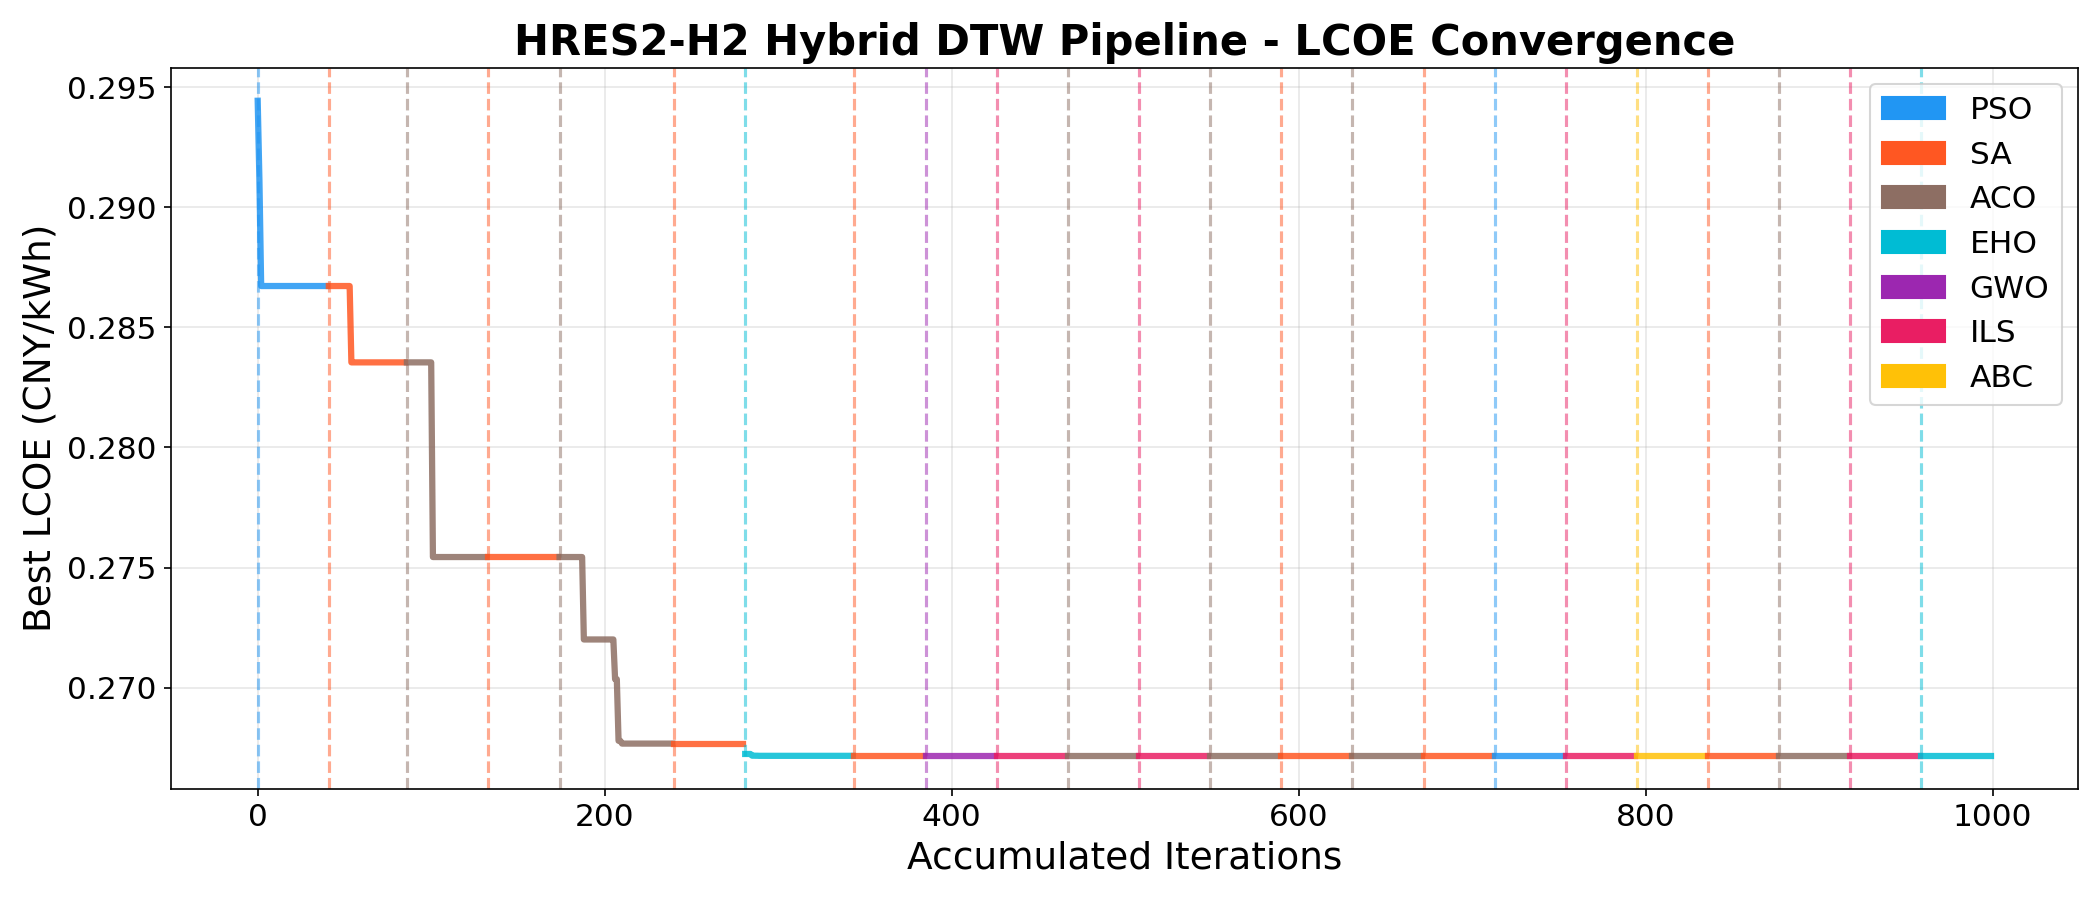
\includegraphics[width=0.85\textwidth]{figures/hres2_dtw_convergence.png}
\caption{DTW Framework convergence trajectory on HRES2-H2.}
\label{fig:hres2_dtw_conv}
\end{figure}

% --- DTW DELTA ---
\begin{figure}[H]
\centering
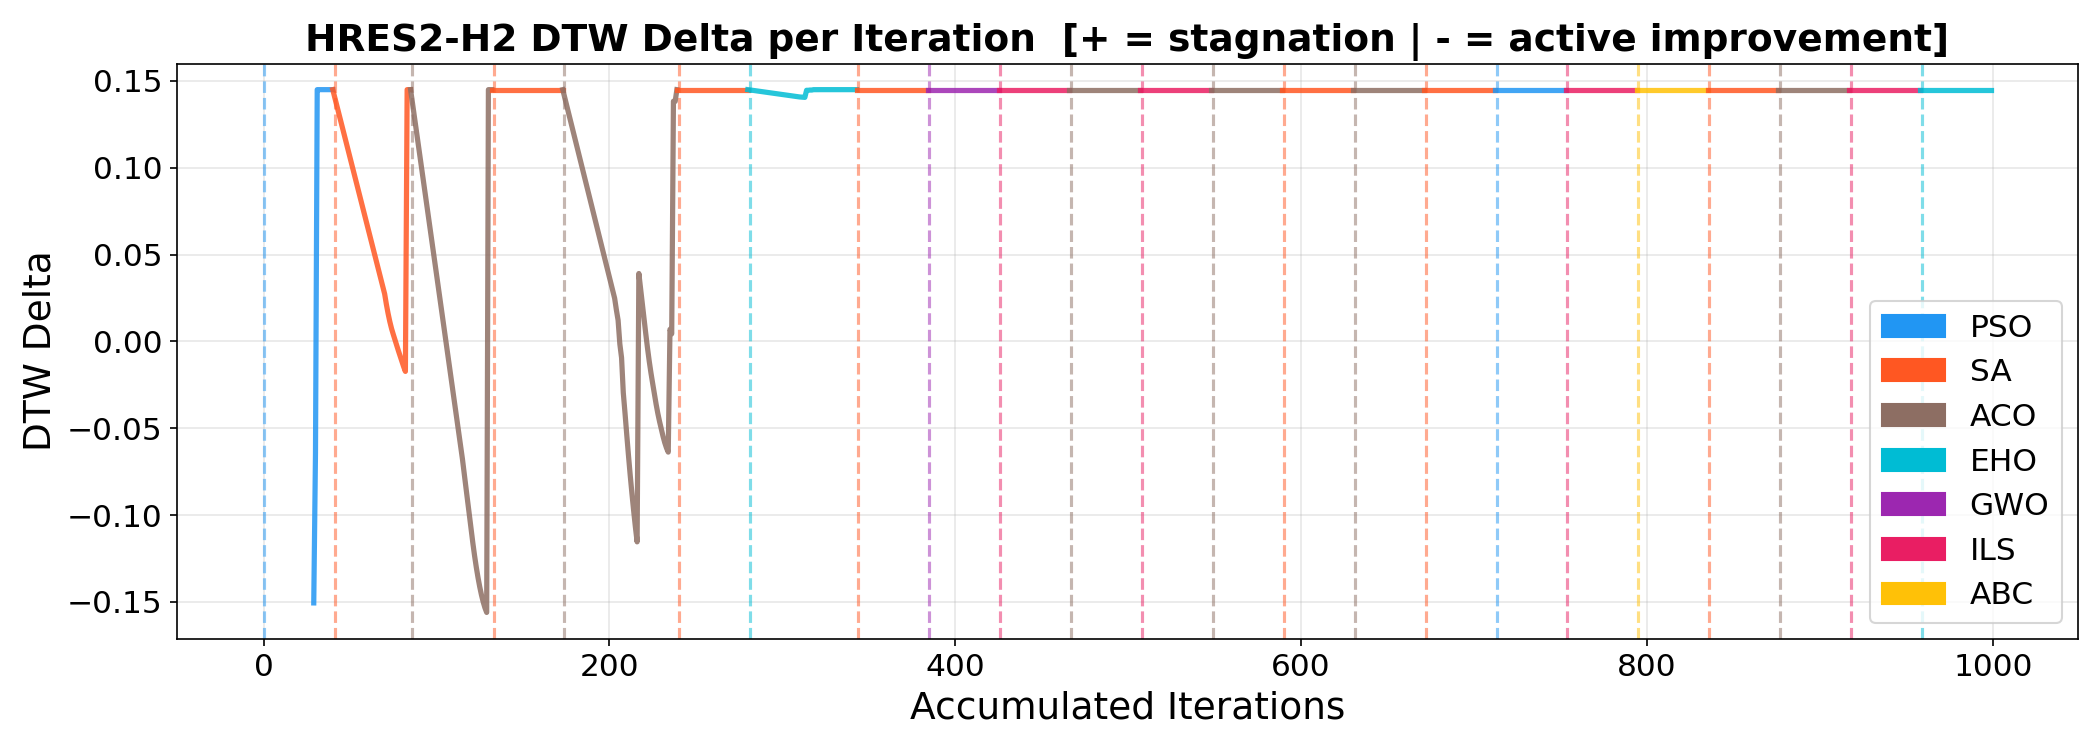
\includegraphics[width=0.85\textwidth]{figures/hres2_dtw_delta.png}
\caption{DTW Framework elastic divergence metric profil on HRES2-H2.}
\label{fig:hres2_dtw_delta}
\end{figure}

% --- DDTW CONVERGENCE ---
\begin{figure}[H]
\centering
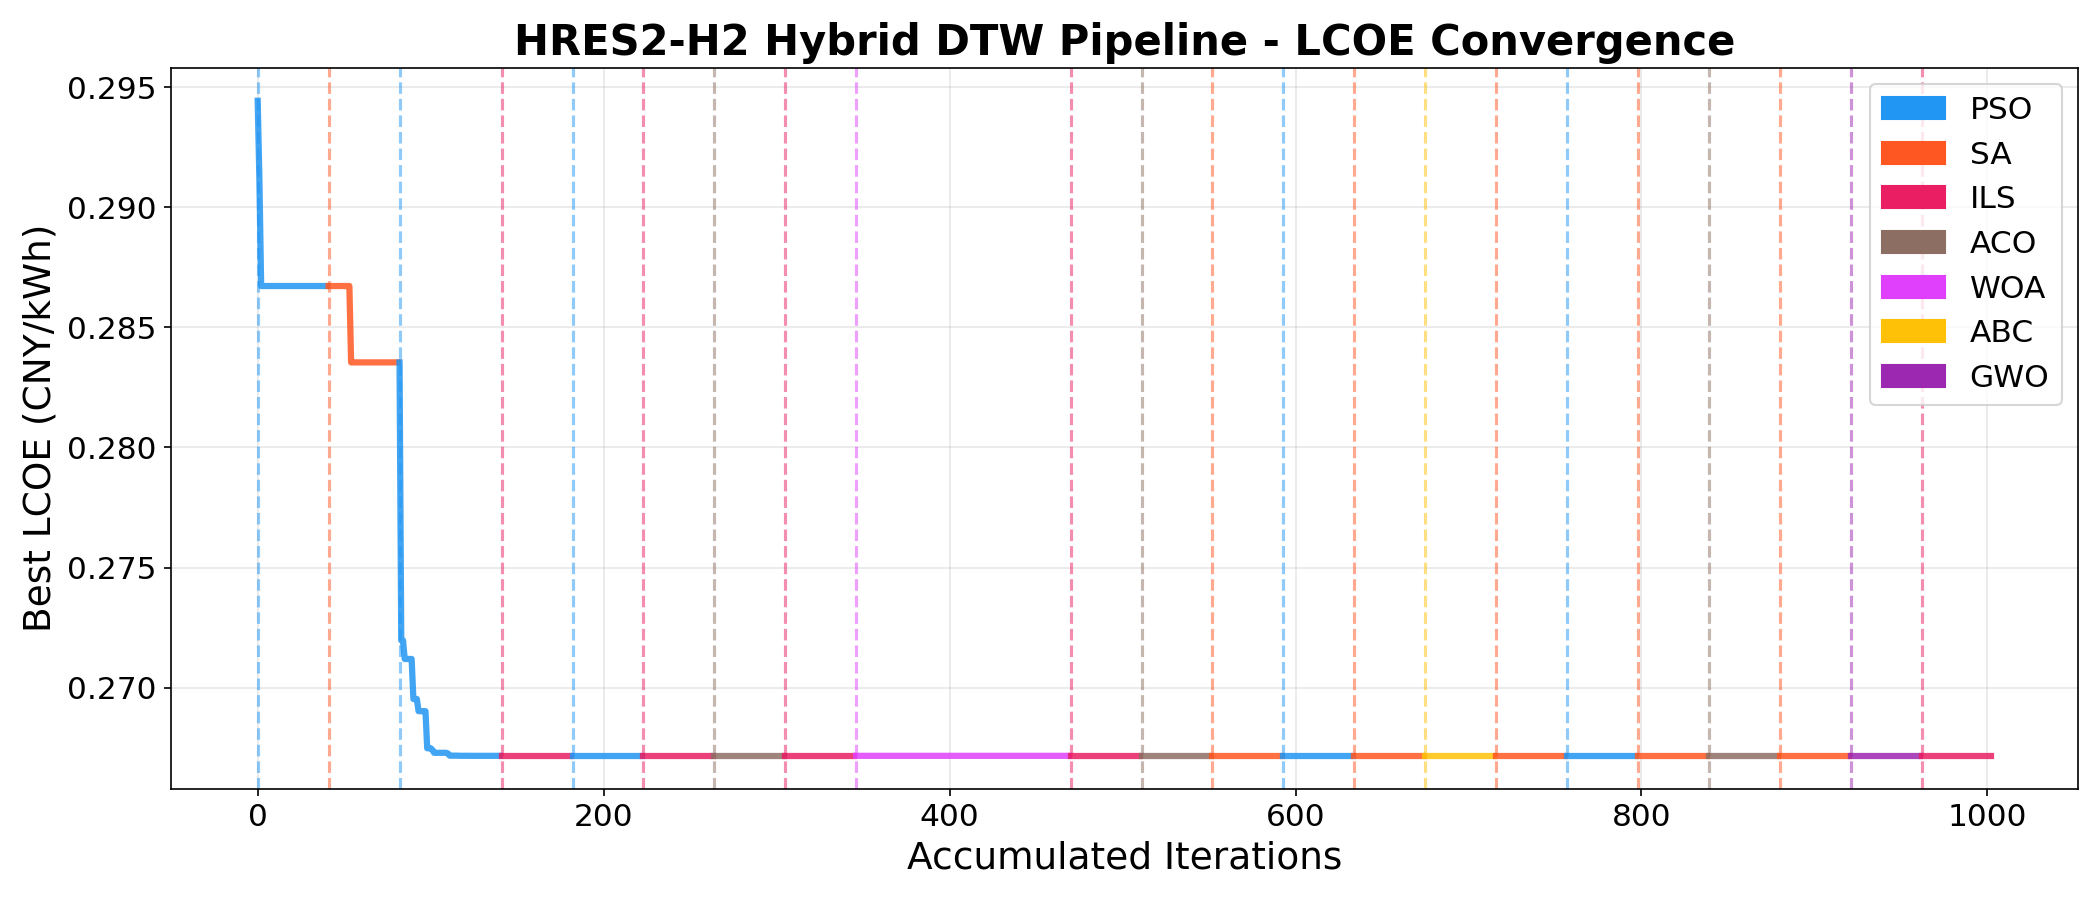
\includegraphics[width=0.85\textwidth]{figures/hres2_ddtw_convergence.png}
\caption{DDTW Framework convergence trajectory on HRES2-H2.}
\label{fig:hres2_ddtw_conv}
\end{figure}

% --- DDTW DELTA ---
\begin{figure}[H]
\centering
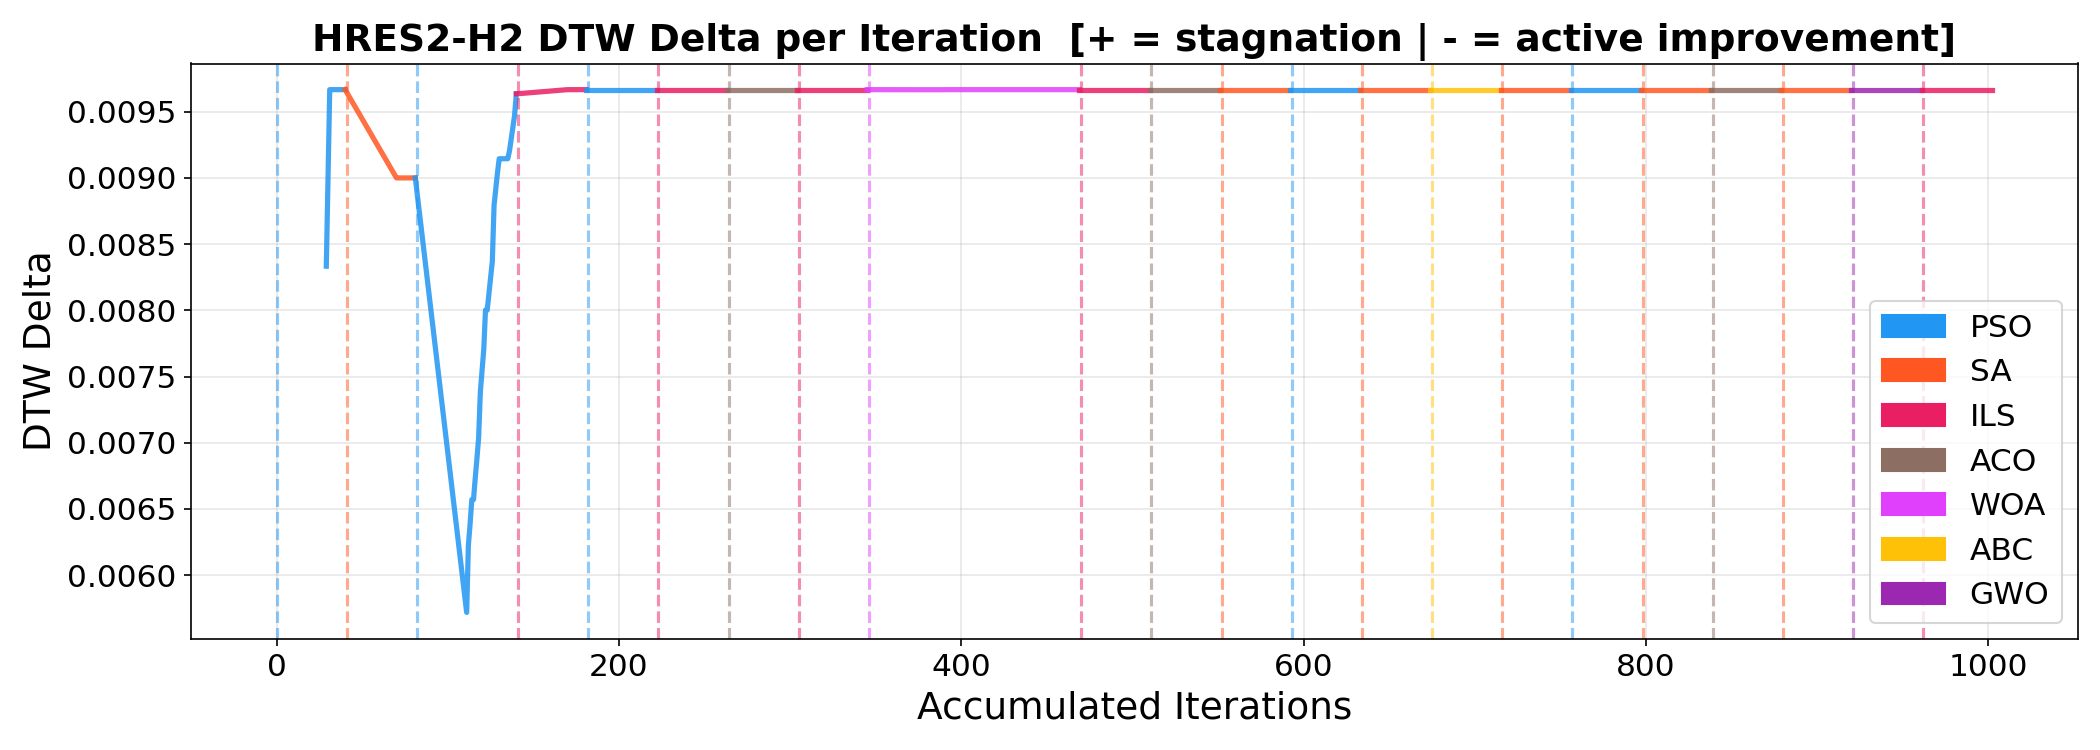
\includegraphics[width=0.85\textwidth]{figures/hres2_ddtw_delta.png}
\caption{DDTW Framework derivative-based divergence metric profile on HRES2-H2.}
\label{fig:hres2_ddtw_delta}
\end{figure}

As shown in Figures~\ref{fig:hres2_dtw_conv} and \ref{fig:hres2_ddtw_conv}, both modalities exhibit rapid initial descent during the exploratory swarm phase ($t < 150$), followed by characteristic convergence plateaus where standalone metaheuristics typically stall. In Figure~\ref{fig:hres2_dtw_delta}, the DTW metric $\Delta$ effectively tracks the divergence between the sliding fitness window and synthetic reference baselines, triggering rotational solver switches whenever stagnation is confirmed. Similarly, Figure~\ref{fig:hres2_ddtw_delta} demonstrates how the derivative-based DDTW monitor detects subtle slope flattening, enabling earlier transitions between global exploration and local exploitation to reach the best observed objective value ($0.267159$~CNY/kWh).








\section{Cross-Domain Inferential Statistical Analysis}
\label{sec:statistical-analysis-final}

This section evaluates whether the proposed DTW- and DDTW-driven hybrid
frameworks differ significantly from the standalone metaheuristics in the
three experimental domains: the Multidimensional Knapsack Problem (MKP), the
IEEE CEC2022 continuous benchmark, and the HRES2--H2 engineering case. Each
method was evaluated over 31 stochastic runs. In MKP and CEC2022, corresponding
run indices followed the same seed schedule and were treated as matched
experimental blocks. In HRES2--H2, this pairing is documented only for the
direct DTW--DDTW comparison; the standalone-method samples were therefore
treated as independent.

\subsection{Statistical protocol}

Normality was assessed with the Shapiro--Wilk test at $\alpha=0.05$. Since
normality was rejected in a substantial fraction of the framework
distributions, inferential conclusions were based on non-parametric tests. For
the matched MKP and CEC2022 observations, the Friedman test was used as the
omnibus comparison and the two-sided Wilcoxon signed-rank test was used for
pairwise contrasts. The HRES2--H2 hybrid--baseline comparisons used the
two-sided Mann--Whitney $U$ test because the archived baseline samples are
independent rather than matched. Family-wise error was controlled with Holm's
step-down procedure: over the six MKP configuration contrasts, over the seven
hybrid--baseline tests within each MKP instance, over the five
hybrid--baseline tests within each CEC2022 function, over the 12 direct
CEC2022 DTW--DDTW contrasts, and separately over the ten HRES2--H2 comparisons
of each framework variant. A comparison was considered significant when
$p_{\mathrm{Holm}}<0.05$.

The direction of every pairwise result is reported from the perspective of
the hybrid framework. Thus, W/T/L denotes a significant hybrid win, a
non-significant tie, or a significant hybrid loss, respectively. Larger
fitness is better in MKP, whereas smaller objective values are better in
CEC2022 and HRES2--H2. Raw objective values from different MKP instances or
CEC2022 functions were not pooled because they have different scales. Global
conclusions instead use normalized gaps, within-problem ranks, and aggregated
within-problem pairwise decisions.

\subsection{Multidimensional Knapsack Problem}
\label{sec:final-stat-mkp}

The MKP analysis covered the first instance of each of the nine Chu--Beasley
families and four framework configurations: DTW--1K, DDTW--1K, DTW--3K, and
DDTW--3K. Shapiro--Wilk rejected normality in 14 of the 36
instance--configuration distributions. Therefore, the comparison among the
four configurations used the mean percentage gap to the best known solution
(BKS), with lower values indicating better performance.

The Friedman test detected a significant difference among the four
configurations ($\chi_F^2=24.0667$, $p=2.419\times10^{-5}$). DTW--3K obtained
the best mean rank (1.22), followed by DDTW--3K (1.78), DTW--1K (3.11), and
DDTW--1K (3.89). All six paired configuration comparisons remained
significant after Holm correction (Table~\ref{tab:final-mkp-config-tests}).
Increasing the budget from 1K to 3K reduced the average gap from 2.237\% to
1.805\% for DTW (19.3\% relative reduction) and from 2.391\% to 1.876\% for
DDTW (21.5\% relative reduction).

\begin{table}[htbp]
\centering
\caption{Paired Wilcoxon comparisons of the mean MKP gap across the nine
instances. Holm adjustment was applied to the six contrasts.}
\label{tab:final-mkp-config-tests}
\begin{tabular}{lrr}
\toprule
Configuration contrast & Raw $p$ & $p_{\mathrm{Holm}}$ \\
\midrule
DTW--1K vs. DDTW--1K   & 0.027344 & 0.039063 \\
DTW--1K vs. DTW--3K    & 0.003906 & 0.023438 \\
DTW--1K vs. DDTW--3K   & 0.003906 & 0.023438 \\
DDTW--1K vs. DTW--3K   & 0.003906 & 0.023438 \\
DDTW--1K vs. DDTW--3K  & 0.003906 & 0.023438 \\
DTW--3K vs. DDTW--3K   & 0.019531 & 0.039063 \\
\bottomrule
\end{tabular}
\end{table}

Within each instance and campaign, the hybrid framework was compared with
PSO, GWO, WOA, EHO, ACO, GA, and SA. All 36 per-instance Friedman tests were
significant. Table~\ref{tab:final-mkp-wtl} aggregates the Holm-adjusted
decisions without mixing raw fitness values across instances.

\begin{table}[htbp]
\centering
\caption{MKP wins/ties/losses of each hybrid configuration against the seven
standalone metaheuristics over nine instances. Each cell is W/T/L from the
hybrid perspective.}
\label{tab:final-mkp-wtl}
\small
\resizebox{\textwidth}{!}{%
\begin{tabular}{lrrrrrrrr}
\toprule
Configuration & PSO & GWO & WOA & EHO & ACO & GA & SA & Total \\
\midrule
DTW--1K  & 9/0/0 & 5/4/0 & 6/3/0 & 8/1/0 & 7/2/0 & 5/1/3 & 1/8/0 & \textbf{41/19/3} \\
DDTW--1K & 9/0/0 & 5/4/0 & 5/4/0 & 9/0/0 & 7/2/0 & 4/2/3 & 1/4/4 & \textbf{40/16/7} \\
DTW--3K  & 9/0/0 & 5/3/1 & 5/3/1 & 9/0/0 & 7/2/0 & 5/1/3 & 1/6/2 & \textbf{41/15/7} \\
DDTW--3K & 9/0/0 & 5/3/1 & 5/3/1 & 9/0/0 & 7/2/0 & 4/1/4 & 1/6/2 & \textbf{40/15/8} \\
\bottomrule
\end{tabular}%
}
\end{table}

The hybrids were particularly consistent against PSO, EHO, and ACO. GA was
the strongest competitor, producing significant advantages in three
instances against DTW--1K, three against DDTW--1K, three against DTW--3K, and
four against DDTW--3K. SA was frequently statistically tied with the hybrid
and was significantly better in selected 1K and 3K campaigns. Consequently,
the MKP evidence supports robust portfolio performance, while it does not
support a claim of universal superiority over every standalone method.

\subsection{IEEE CEC2022 continuous benchmark}
\label{sec:final-stat-cec2022}

The final CEC2022 analysis uses the completed DTW job 19070 and DDTW job
19066. Each campaign compared its hybrid control with PSO, GWO, WOA, EHO, and
ACO on functions F1--F12 at $D=10$. Shapiro--Wilk rejected normality for the
hybrid in 10 of the 12 functions in each campaign. All 12 per-function
Friedman tests were significant for both DTW and DDTW, demonstrating that the
six algorithms did not have equivalent performance distributions on any
function.

Ranks were calculated within each function and then averaged across the 12
functions. The hybrid obtained the best aggregate rank in both campaigns:
2.323 for DTW and 2.358 for DDTW (Table~\ref{tab:final-cec-ranks}). This
within-function aggregation avoids distortion from the different CEC2022
objective scales and bias terms.

\begin{table}[htbp]
\centering
\caption{Aggregate mean ranks across the 12 CEC2022 functions. Lower ranks
indicate better performance.}
\label{tab:final-cec-ranks}
\begin{tabular}{lrr}
\toprule
Algorithm & DTW campaign & DDTW campaign \\
\midrule
Hybrid framework & \textbf{2.323} & \textbf{2.358} \\
EHO              & 3.156 & 3.142 \\
ACO              & 3.257 & 3.269 \\
PSO              & 3.372 & 3.364 \\
GWO              & 3.616 & 3.598 \\
WOA              & 5.277 & 5.269 \\
\bottomrule
\end{tabular}
\end{table}

The Holm-adjusted pairwise outcomes are summarized in
Table~\ref{tab:final-cec-wtl}. DTW achieved 38 significant wins, 16 ties, and
6 losses in 60 comparisons, whereas DDTW achieved 37 wins, 19 ties, and 4
losses. WOA showed the clearest framework advantage, with 11 wins and one tie
for each alignment variant. ACO was the most competitive baseline, accounting
for three DTW losses and two DDTW losses.

\begin{table}[htbp]
\centering
\caption{CEC2022 Holm-adjusted Wilcoxon outcomes against the standalone
metaheuristics. Counts are W/T/L from the hybrid perspective over 12
functions.}
\label{tab:final-cec-wtl}
\begin{tabular}{lrr}
\toprule
Comparator & DTW & DDTW \\
\midrule
PSO & 7/3/2  & 6/5/1 \\
GWO & 8/4/0  & 8/4/0 \\
WOA & 11/1/0 & 11/1/0 \\
EHO & 7/4/1  & 6/5/1 \\
ACO & 5/4/3  & 6/4/2 \\
\midrule
Total & \textbf{38/16/6} & \textbf{37/19/4} \\
\bottomrule
\end{tabular}
\end{table}

The direct paired DTW--DDTW comparison was also conducted independently for
each function and adjusted across the 12 tests. None of the contrasts remained
significant after Holm correction ($0/12$). DTW had the lower mean at full
precision on seven functions and DDTW on five, but this descriptive difference
does not establish statistical superiority of either alignment strategy.
Therefore, the CEC2022 results support broad competitiveness against the
standalone methods and a landscape-dependent balance between DTW and DDTW.

\subsection{HRES2--H2 engineering case}
\label{sec:final-stat-hres2}

The engineering experiment compared each hybrid with PSO, GWO, WOA, EHO,
ACO, ILS, SA, TS, and VNS using the levelized cost of electricity (LCOE)
as the common minimization metric. Each objective evaluation simulated 8,760
hourly dispatch steps over the same fixed synthetic weather profile. The
Shapiro--Wilk test rejected normality for both hybrid LCOE distributions
($p<10^{-11}$).

The HRES2--H2 archive does not preserve the individual baseline observations
or a common-seed correspondence between each baseline and the hybrid. Thus,
the archived row-wise Friedman and Wilcoxon calculations are not used as
inferential evidence here. Instead, Table~\ref{tab:final-hres-tests} reports
the archived mean LCOE and the archived two-sided Mann--Whitney $p$-values
after a reproducible Holm adjustment over the ten comparisons in each
campaign. Every baseline had a higher mean LCOE than its hybrid control, and
all 20 distributional contrasts remained significant after adjustment. This
yields a 10/0/0 win/tie/loss record for each framework variant.

\begin{table}[htbp]
\centering
\caption{HRES2--H2 comparison against standalone metaheuristics. The reported
$p$-values are two-sided Mann--Whitney values adjusted by Holm over the ten
independent-sample comparisons of each framework variant.}
\label{tab:final-hres-tests}
\scriptsize
\resizebox{\textwidth}{!}{%
\begin{tabular}{lrrrr}
\toprule
& \multicolumn{2}{c}{DTW campaign} & \multicolumn{2}{c}{DDTW campaign} \\
\cmidrule(lr){2-3}\cmidrule(lr){4-5}
Method & Mean LCOE & $p_{\mathrm{Holm}}^{\mathrm{MW}}$ & Mean LCOE & $p_{\mathrm{Holm}}^{\mathrm{MW}}$ \\
\midrule
Hybrid control & \textbf{0.267160} & -- & \textbf{0.267160} & -- \\
GWO & 0.268066 & $6.384\times10^{-10}$ & 0.268395 & $2.272\times10^{-9}$ \\
VNS & 0.267806 & $2.232\times10^{-10}$ & 0.267806 & $1.090\times10^{-9}$ \\
TS  & 0.267188 & $1.242\times10^{-10}$ & 0.267184 & $6.880\times10^{-10}$ \\
ILS & 0.267184 & $1.242\times10^{-10}$ & 0.267183 & $6.880\times10^{-10}$ \\
ACO & 0.273288 & $7.639\times10^{-7}$  & 0.273617 & $1.316\times10^{-5}$ \\
PSO & 0.277289 & $1.285\times10^{-2}$  & 0.280068 & $1.573\times10^{-3}$ \\
WOA & 0.277227 & $2.373\times10^{-5}$  & 0.276477 & $1.797\times10^{-2}$ \\
EHO & 0.277728 & $4.333\times10^{-7}$  & 0.278524 & $1.431\times10^{-8}$ \\
SA  & 0.286431 & $8.591\times10^{-11}$ & 0.290062 & $9.340\times10^{-11}$ \\
\bottomrule
\end{tabular}%
}
\end{table}

The archive stores per-run LCOE values to six decimal places. On these values,
the paired same-seed Wilcoxon test did not detect a difference between DTW and
DDTW ($p=0.593$). The mean difference was only $7.42\times10^{-7}$ CNY/kWh,
below the reporting precision.
Accordingly, the experiment provides no evidence of an LCOE difference between
the variants; this non-significant result is not, by itself, a formal
equivalence test. The conclusion is restricted to the fixed synthetic weather
profile and to LCOE. Moreover, the standalone-method archive retains summary
statistics and test outputs, but not the individual baseline LCOE observations
or per-run LCOH, hydrogen-production, feasibility, and component-sizing
records.

\subsection{Cross-domain interpretation}
\label{sec:final-stat-synthesis}

The three domains provide complementary evidence. In MKP, the 3K budget
significantly improves solution quality and DTW--3K has the best configuration
rank, although GA and SA remain competitive on selected instances. In
CEC2022, each hybrid has the best aggregate rank in its own campaign and wins
most pairwise comparisons, but neither DTW nor DDTW is significantly superior
to the other. In HRES2--H2, both hybrids have lower mean LCOE than all ten
standalone methods, with significant independent-sample distributional
differences after Holm correction, while the paired test detects no
DTW--DDTW difference.
Overall, the results support the robustness of the adaptive portfolio across
discrete, continuous, and engineering optimization, without implying universal
dominance on every individual problem or formal equivalence of DTW and DDTW.











% -----------------------------------------------------------------------------
% Final discussion of the MKP, CEC2022, and HRES2--H2 results.
% This is an input fragment, not a standalone LaTeX document.
% Required packages: amsmath, booktabs, graphicx, and array.
% -----------------------------------------------------------------------------

\section{Discussion}
\label{sec:discussion-final}

The experiments provide consistent evidence that the proposed
DTW/DDTW-driven rotational framework is a robust way to exploit a portfolio of
metaheuristics across discrete, continuous, and engineering optimization
problems (Tables~\ref{tab:final-mkp-wtl}, \ref{tab:final-cec-wtl}, and
\ref{tab:final-hres-tests}). Its main benefit is not universal dominance on every problem, but a
reduction in dependence on the choice of a single standalone solver. This
distinction is important. In MKP, the framework accumulated between 40 and 41
significant wins across 63 baseline comparisons, depending on the
configuration, but it also incurred between 3 and 8 significant losses. In
CEC2022, DTW and DDTW achieved the best aggregate ranks among the six evaluated
methods, although specialized baselines remained preferable on some functions.
In HRES2--H2, both variants produced lower mean LCOE than all ten standalone
methods and all distributional comparisons remained significant after Holm
correction. Taken together, these findings support the framework as an
effective portfolio controller, while ruling out the stronger claim that it
must outperform every constituent algorithm on every landscape.


\subsection{MKP: budget effect and DTW--3K}
\label{sec:discussion-mkp}

The MKP results in Tables~\ref{tab:mkp_dtw_1k}--\ref{tab:mkp_ddtw_3k}
provide the clearest discrimination among the four framework configurations.
The global Friedman test was significant
($\chi_F^2=24.0667$, $p=2.419\times10^{-5}$), and all six paired configuration
contrasts remained significant after Holm correction. DTW--3K obtained the
best mean rank (1.22) and the lowest average normalized gap (1.805\%), followed
by DDTW--3K (rank 1.78; gap 1.876\%), DTW--1K (rank 3.11; gap 2.237\%), and
DDTW--1K (rank 3.89; gap 2.391\%); the corrected pairwise results are reported
in Table~\ref{tab:final-mkp-config-tests}. DTW--3K also achieved the lowest mean gap in
seven of the nine selected instances, while DDTW--3K was best in
\texttt{mknapcb2} and \texttt{mknapcb9}. Accordingly, DTW--3K is the best
supported configuration for this MKP test set.

The budget effect is both statistically and practically relevant. Increasing
the search from 1,000 to 3,000 iterations reduced the average gap by 19.3\% for
DTW and 21.5\% for DDTW. This result indicates that the hybrid had not exhausted
its useful search dynamics at 1,000 iterations. The corresponding mean number
of switches increased from 7.85 to 26.70 for DTW and from 16.43 to 26.96 for
DDTW. However, switch frequency and solution quality should not be conflated:
the logs show that more switching occurred under the longer budget, but they do
not demonstrate that every individual rotation generated an improvement.

At 1K, DDTW switched approximately twice as often as DTW while obtaining a
higher mean gap. One plausible explanation is that derivative-based alignment
is more sensitive to short changes around discrete plateaus and therefore
triggers more rotations without necessarily improving the incumbent solution.
By contrast, the absolute level information retained by DTW may be useful when
fitness trajectories contain long plateaus separated by discrete jumps. This
is a mechanism-level hypothesis, not a causal conclusion: it should be tested
with event-level analyses linking each switch to subsequent improvement, and
with controlled experiments that vary the monitoring window and patience
parameters.

The improved 3K performance also entails a computational trade-off. The
observed mean campaign times increased from 306.94 to 756.11 seconds for DTW
and from 256.43 to 682.21 seconds for DDTW. These measurements combine the
larger evaluation budget, solver cost, machine conditions, and monitoring
overhead; consequently, they quantify the empirical quality--time trade-off of
the campaigns but do not isolate the cost of DTW or DDTW itself. A fair overhead
study would compare identical solver trajectories with and without the monitor
under controlled hardware and evaluation counts.

\subsection{CEC2022: competitive but not universal}
\label{sec:discussion-cec2022}

The CEC2022 experiments in Table~\ref{tab:cec2022_results} show that the
framework generalizes beyond the discrete setting. DTW and DDTW achieved the
best aggregate mean ranks among the six evaluated algorithms, 2.323 and 2.358,
respectively (Table~\ref{tab:final-cec-ranks}). Their Holm-adjusted W/T/L
totals were 38/16/6 for DTW and 37/19/4 for DDTW across 60
hybrid--baseline comparisons. All 12 function-wise Friedman tests were
significant in each campaign, confirming that algorithm choice affected the
observed objective values. The framework therefore offers broad competitive
coverage, but the losses and ties show that no single hybrid variant dominated
the entire suite.

This landscape dependence is also visible in the descriptive results. DTW
reported the best hybrid mean on F6, F7, F8, and F11, whereas DDTW did so on
F10 and F12; on other functions, a standalone method could retain the best
mean. At the best-run level, both variants reached the official optimum on F1,
F5, and F11. Best-run results demonstrate attainable performance but are more
sensitive to stochastic selection than distributions over 31 runs, so the
rank and paired-test results should carry greater inferential weight. The large
dispersion on F6 (standard deviations of approximately 1,821.985 for DTW and
1,942.164 for DDTW) further illustrates why isolated best values are
insufficient to characterize robustness.

The direct DTW--DDTW comparison found no Holm-significant difference on any of
the 12 functions. DTW had the lower unrounded mean on seven functions and a
slightly lower average normalized mean gap (10.281\% versus 10.501\%), but the
evidence does not support declaring one alignment modality generally superior
for CEC2022. Equally, a non-significant result is not evidence of equivalence.
An equivalence or non-inferiority design with a prespecified practically
relevant margin would be required to claim that the two variants are
interchangeable.

Interestingly, switching activity in CEC2022 was much lower than in the MKP
3K and HRES2--H2 campaigns: DTW averaged 6.20 switches and DDTW 6.01, with a
range of four to ten. Because the stopping budgets and search spaces differ,
these raw counts are not directly comparable as rates. Nevertheless, their
variation across functions and domains is consistent with a data-dependent
trigger rather than a fixed rotation timetable. A future analysis should
normalize events by eligible monitoring iterations and relate them to
post-switch improvement, diversity recovery, and solver identity.

\subsection{HRES2--H2: statistical evidence and engineering relevance}
\label{sec:discussion-hres2}

In the engineering case, both variants converged to almost the same economic
region (Table~\ref{tab:hres2_metrics}). Their archived mean LCOE was 0.267160 CNY/kWh, with best values of
0.267159 CNY/kWh. The associated mean LCOH values were 17.631382 CNY/kg for DTW
and 17.631312 CNY/kg for DDTW. The best designs also shared the same reported
capacity pattern: approximately 174.47 MW of wind, 25.53 MW of photovoltaic
generation, 70 MW of electrolyzers, and a 50 MW/4 h battery, with annual
hydrogen production of approximately $8.86\times10^6$ kg. The renewable-share
constraint was active at, or very near, its 20\% upper bound. This boundary
solution indicates that the optimizer exploited the allowable grid support to
minimize cost under the stated formulation.

Against the ten standalone methods, all baseline mean LCOE values were higher,
and all Mann--Whitney comparisons in Table~\ref{tab:final-hres-tests} remained significant after Holm correction,
yielding W/T/L $=10/0/0$ for each framework variant. The magnitude of the
improvement was nevertheless heterogeneous. The relative reduction in mean
LCOE ranged from approximately 0.009\% against ILS to 6.73\% against SA for
DTW, and from approximately 0.009\% against ILS to 7.90\% against SA for
DDTW. Therefore, statistical significance should not be interpreted as uniform
engineering importance. Against ILS and TS, the absolute advantage is very
small and becomes statistically detectable because the distributions are
highly concentrated; against weaker baselines such as SA, the economic
difference is materially larger.

The direct same-seed comparison between DTW and DDTW produced a mean LCOE
difference of only $7.419\times10^{-7}$ CNY/kWh and a two-sided Wilcoxon
$p=0.593$. The data therefore do not detect a performance difference between
the alignment variants in this case. They do not establish formal equivalence,
particularly because objective values were archived at six decimal places and
the between-run dispersion was extremely small. The narrow distributions may
reflect stable behavior of the framework, but they may also arise from the
low-dimensional constrained basin, the deterministic dispatch rules, and the
use of one fixed weather and load profile.

The HRES2--H2 interpretation must also remain aligned with the implemented
system boundary. The case models grid-connected wind, photovoltaic generation,
an electrolyzer, and a battery for annual hydrogen production. It does not
include a hydrogen storage tank, fuel-cell reconversion, or a minimum hydrogen
demand constraint. Consequently, the results validate the optimizer for the
specified wind--PV--electrolyzer--battery sizing and dispatch problem, not for
every configuration commonly described as a complete hydrogen-storage
microgrid. Robust engineering conclusions will require multiple weather and
price years, demand scenarios, technology-cost trajectories, and uncertainty
or reliability constraints.

\subsection{What can be inferred from the switching dynamics}
\label{sec:discussion-switching}

The switch counts differed substantially by domain and budget: 7.85 and 16.43
for DTW--1K and DDTW--1K in MKP; 26.70 and 26.96 under the 3K budget; 6.20 and
6.01 in CEC2022; and 21.00 and 21.68 in HRES2--H2. This heterogeneity is
compatible with the intended behavior of an adaptive controller whose trigger
depends on the recent trajectory rather than on a fixed number of iterations.
The similarity between DTW and DDTW in CEC2022 and HRES2--H2 also suggests that
both representations identified comparable stagnation structure in those
campaigns, whereas their larger separation in MKP--1K points to a stronger
effect of trajectory representation on discrete plateaus.

The synchronized HRES2--H2 convergence and diagnostic profiles in
Figures~\ref{fig:hres2_dtw_conv}--\ref{fig:hres2_ddtw_delta} visually connect
fitness plateaus with the monitor signals and solver handoffs. These plots are
useful for explaining the operating principle, but they correspond to selected
best-run traces rather than an average trajectory over 31 runs. They should
therefore be interpreted as mechanism illustrations, not as independent
evidence that the same temporal sequence occurred in every run.

These counts remain diagnostic rather than causal evidence. They do not state
which solver was entered or left, whether diversity increased, how long the
benefit persisted, or whether an improvement would have occurred without the
switch. A stronger causal analysis would compare the observed policy with
fixed-period rotation, random rotation, a no-switch portfolio, and the same
solvers run independently under equal evaluation budgets. Event studies could
then estimate the change in improvement rate immediately before and after a
trigger and identify which transitions contribute most to performance.

\subsection{Role of shared elitist memory}
\label{sec:discussion-memory}

The framework transfers the incumbent elite solution across solver rotations.
This design is important because it protects the best solution found so far
while allowing the active search dynamics to change. It offers a plausible
explanation for why rotation can diversify the search without sacrificing
accumulated progress, especially in MKP and HRES2--H2 where returning to a
previously identified high-quality region is valuable. At the same time,
aggressive elitist transfer can reduce effective diversity if each solver is
reinitialized too close to the same incumbent. The current results demonstrate
the performance of the complete framework but do not separate the effects of
the monitor, solver rotation, and elite transfer. A factorial ablation with and
without memory, adaptive triggering, and portfolio diversity is needed for
component-level attribution.


\section{Conclusions}
\label{sec:conclusions}

This work proposed a trajectory-driven collaborative metaheuristic framework in which Dynamic Time Warping (DTW) and Derivative Dynamic Time Warping (DDTW) are used to monitor the temporal pattern of the recent best-so-far fitness trajectory. Rather than relying on fixed iteration budgets, scalar stagnation counters, or learned decision policies, the framework detects persistent search plateaus by aligning a sliding fitness window against synthetic progress and stagnation baselines under Sakoe--Chiba band constraints. Stagnation decisions are governed by run-relative empirical percentiles and a confirmation patience filter, triggering solver rotation between complementary population-based and trajectory-based pools with elitist memory injection.

The framework was evaluated over 31 independent runs across three structurally distinct optimization domains. In the discrete Multidimensional Knapsack Problem (MKP), the extended-budget configuration (DTW--3K) achieved the best mean rank (1.22) and reduced the average optimality gap by up to 21.5\%, accumulating 41 significant wins across 63 baseline comparisons. In the continuous IEEE CEC2022 benchmark ($D=10$), both DTW and DDTW attained the top aggregate Friedman ranks (2.323 and 2.358, respectively), with combined win/tie/loss records of 38/16/6 and 37/19/4 against five standalone population-based methods. In the HRES2--H2 green hydrogen microgrid sizing problem, both variants converged to the same optimal configuration with 100\% constraint feasibility, minimal mean LCOE (0.267160 CNY/kWh), and negligible run-to-run variance ($\sigma \approx 10^{-6}$), significantly outperforming all ten standalone baselines after Holm correction ($p_{\mathrm{Holm}} < 0.05$). No significant difference was detected between DTW and DDTW in any domain after multiplicity adjustment.

These results support two main conclusions. First, explicit trajectory-pattern analysis via elastic alignment provides a viable, model-free, and less sensitive to changes in objective scale feedback signal for governing solver switching in collaborative metaheuristic frameworks. The same monitor parameterization operated across fitness scales spanning several orders of magnitude without manual recalibration. Second, trajectory-driven portfolio rotation reduces the dependence on selecting a single optimal solver: the framework achieved competitive or superior performance across heterogeneous landscapes without requiring any individual constituent algorithm to dominate universally.

Several limitations define the scope of these conclusions. The MKP evaluation covers nine Chu--Beasley instances; CEC2022 was tested only at $D=10$; and the HRES2--H2 case uses a single synthetic annual weather profile. The monitor hyperparameters (window length, percentiles, patience) were fixed throughout all experiments and were not systematically varied in a sensitivity analysis. Additionally, the present design does not include a no-monitor ablation or a fixed-rotation control, which would be necessary to isolate the contribution of each framework component.

Several promising directions emerge from this work:
\begin{itemize}
    \item \textbf{DTW-driven inter-algorithm communication for adaptive parameter control.} The current framework uses the stagnation signal exclusively to trigger solver switching. A natural extension is to exploit the DTW/DDTW distance metrics as a continuous feedback channel that modulates internal algorithmic parameters (e.g., inertia weight in PSO, mutation rate in GA, cooling schedule in SA, or neighborhood depth in VNS) without necessarily replacing the active solver. This would enable a finer-grained adaptive response in which the trajectory shape informs both \emph{when} to switch algorithms and \emph{how} to reconfigure the current one.
    \item \textbf{Extended HRES2--H2 microgrid model.} The present engineering case study considers a simplified WPEB system without explicit hydrogen storage tanks or fuel-cell re-electrification. Future versions should incorporate a full hydrogen storage and fuel-cell subsystem, multi-year stochastic meteorological scenarios, degradation models for PV panels and electrolyzers, and time-varying electricity tariffs. A systematic evaluation of the applicability, flexibility, and limitations of the proposed framework under increasingly realistic HRES--H$_2$ configurations would help identify the critical problem characteristics and constraints that most influence algorithmic performance and solution quality.
    \item \textbf{Multi-objective optimization.} Extending the trajectory-driven coordination to multi-objective domains (e.g., using Pareto-front convergence indicators as the monitored signal) would test the generality of elastic alignment beyond single-objective fitness curves.
    \item \textbf{Sustainability-driven objectives with adaptive $\varepsilon$-constraint.} A natural extension of the HRES--H$_2$ case study is the integration of sustainability metrics such as CO$_2$ emissions minimization and renewable energy fraction maximization into the optimization framework. Adaptive $\varepsilon$-constraint strategies could serve as lightweight alternatives to fully multi-objective formulations, enabling scalable trade-off management between economic and environmental objectives with limited computational overhead.
    \item \textbf{Lightweight ANN-based dynamic parameter adaptation.} The current DTW/DDTW monitor governs solver switching but does not modify the internal configuration of the active algorithm. Incorporating resource-constrained neural network components (e.g., small MLPs or single-layer autoencoders) to dynamically adapt key algorithmic parameters---including population size, termination criteria, and solution generation strategies---based on trajectory-derived features would enable a learned, yet computationally efficient, adaptive layer complementary to the model-free elastic alignment signal.
\end{itemize}

\section*{CRediT authorship contribution statement}
\textbf{First Author:} Conceptualization, Methodology, Software, Writing – original draft, Writing – review \& editing. \textbf{Second Author:} Methodology, Software, Writing – review \& editing. \textbf{Last Author:} Supervision, Methodology, Validation.
\begin{comment}
For transparency, we require corresponding authors to provide co-author contributions to the manuscript using the relevant CRediT roles. The CRediT taxonomy includes 14 different roles describing each contributor’s specific contribution to the scholarly output. The roles are: Conceptualization; Data curation; Formal analysis; Funding acquisition; Investigation; Methodology; Project administration; Resources; Software; Supervision; Validation; Visualization; Roles/Writing - original draft; and Writing - review & editing. Note that not all roles may apply to every manuscript, and authors may have contributed through multiple roles.
\end{comment}


\section*{Declaration of Competing Interest}
The authors declare that they have no known competing financial interests or personal relationships that could have appeared to influence the work reported in this paper.

\section*{Acknowledgements}
Collate acknowledgements in a separate section at the end of the article before the references and do not, therefore, include them on the title page, as a footnote to the title or otherwise. List here those individuals who provided help during the research (e.g., providing language help, writing assistance or proof reading the article, etc.).

\section*{Data availability}
Provide a link to your data if available.

\bibliography{sample}

\end{document}
